\documentclass[a4paper,12pt]{article}

% Основные пакеты
\usepackage[T1, T2A]{fontenc}
\usepackage[utf8]{inputenc}
\usepackage[english, russian]{babel}
\usepackage{geometry}
\usepackage{indentfirst}
\usepackage{graphicx}
\usepackage{wrapfig}
\usepackage{amsmath, amssymb, amsfonts}
\usepackage{braket} 
\usepackage{float}
\usepackage{amsmath}  % для математических окружений
\usepackage{bm}  
% Гиперссылки и цветовые настройки
\usepackage[dvipsnames]{xcolor}
\usepackage[colorlinks]{hyperref}
\hypersetup{
	linkcolor=blue,
	filecolor=magenta,
	urlcolor=cyan
}

\usepackage{listings}
\usepackage{xcolor}

% Цвета
\definecolor{backcolour}{rgb}{0.95,0.95,0.92}
\definecolor{codegreen}{rgb}{0, 0.5, 0}
\definecolor{codegray}{rgb}{0.4, 0.4, 0.4}
\definecolor{codepurple}{rgb}{0.58, 0, 0.82}
\definecolor{keywordcolor}{rgb}{0.0, 0.2, 0.7}
\definecolor{stringcolor}{rgb}{0.6, 0, 0}
\definecolor{framecolor}{rgb}{0.7, 0.7, 0.7}

% Стиль для Mathematica
\lstdefinestyle{python}{
	language=python,
	backgroundcolor=\color{backcolour},
	basicstyle=\ttfamily\small,
	keywordstyle=\color{keywordcolor}\bfseries,
	commentstyle=\color{codegreen}\itshape,
	stringstyle=\color{stringcolor},
	numberstyle=\tiny\color{codegray},
	numbers=left,
	numbersep=5pt,
	breaklines=true,
	breakatwhitespace=false,
	showstringspaces=false,
	keepspaces=true,
	frame=single,
	rulecolor=\color{framecolor},
	frameround=tttt,
	captionpos=b,
	tabsize=2,
	xleftmargin=1em,
	xrightmargin=0.5em
}

% Установить стиль по умолчанию
\lstset{style=python}

% Путь к изображениям
\graphicspath{{./images/}}

% Геометрия страницы
\geometry{left=2cm, right=2cm, bottom=2cm, top=2cm}

\begin{document}
	\begin{titlepage}
		\centering
		\vspace*{1cm}
		
		{\large Министерство науки и высшего образования Российской Федерации}\\
		{\large ФЕДЕРАЛЬНОЕ ГОСУДАРСТВЕННОЕ АВТОНОМНОЕ ОБРАЗОВАТЕЛЬНОЕ УЧРЕЖДЕНИЕ ВЫСШЕГО ОБРАЗОВАНИЯ «НАЦИОНАЛЬНЫЙ ИССЛЕДОВАТЕЛЬСКИЙ УНИВЕРСИТЕТ ИТМО»}\\
		{\large (УНИВЕРСИТЕТ ИТМО)}\\
		
		\vspace{2cm}
		
		{\large Факультет «Систем управления и робототехники»}\\
		
		\vspace{3cm}
		
		\textbf{{\Huge ОТЧЕТ}\\
			{\Huge О ЛАБОРАТОРНОЙ РАБОТЕ №4}}\\
		
		\vspace{1cm}
		
		{\LARGE По дисциплине «Частотные методы»}\\
		{\LARGE на тему: «Линейная фильтрация»}\\
		
		\vspace{3cm}
		
		{\Large Студент:}\\
		Охрименко Ева
		
		\vspace{2cm}
		
		{\Large Преподаватели:}\\
		Догадин Егор Витальевич\\
		Пашенко Артем Витальевич\\
		
		\vspace{3cm}
		{\large г. Санкт-Петербург}\\
		{\large 2025}
		
	\end{titlepage}
	\newpage
	\tableofcontents
	\newpage

	\section{Task. Линейные фильтры}
	\subsection{Фильтр первого порядка}
	
	\subsubsection{Краткое условие}
	Исходный сигнал:
	\[ g(t) = 
	\begin{cases} 
		a, & t \in [t_1, t_2] \\
		0, & t \notin [t_1, t_2]
	\end{cases}
	\]
	
	Зашумленный сигнал:
	\[ u(t) = g(t) + b\xi(t), \quad \xi(t) \sim U[-1,1] \]
	
	Фильтр первого порядка:
	\[ W_1(p) = \frac{1}{Tp + 1} \]
	
	\textbf{Задачи:}
	\begin{itemize}
		\item Построить АЧХ фильтра для заданного $T$
		\item Исследовать влияние $T$ и $a$ на фильтрацию
		\item Построить графики:
		\begin{itemize}
			\item $g(t)$, $u(t)$ и фильтрованного сигнала
			\item Модули Фурье-образов сигналов
			\item Сравнение временных и частотных методов фильтрации
		\end{itemize}
		\item Сделать выводы
	\end{itemize}

	\subsubsection{Предподготовка}
	
	Возьму сигнал 
	\[ g(t) = 
	\begin{cases} 
		4, & t \in [1, 5] \\
		0, & t \notin [1, 5]
	\end{cases}
	\]
	
	Зашумленный сигнал:
	\[ u(t) = g(t) + 0.5\xi(t), \quad \xi(t) \sim U[-1,1] \] - слагаемое с синусом отсутствует.
	
	Пропущу сигнал через фильтр первого порядка
	\[ W_1(p) = \frac{1}{Tp + 1} \]
	
	
	Проведу два этапа исследования:
	
	\begin{enumerate}
		\item При фиксированном $a=4$ исследую влияние постоянной времени $T$ на качество фильтрации для значений $T = [0.5, 0.1, 0.05]\,c$.
		
		\item При фиксированном $T=0.1\,c$ изучу зависимость результатов фильтрации от амплитуды сигнала $a = [0.5, 5, 10]$.
	\end{enumerate}
	
	\subsubsection{АЧХ фильтра}
	
	Приведу графики для выбранных ранее значений \(T\). Также на них я укажу частоту среза \(\omega_0 = \frac{1}{T}\) и  \(W(\omega_0) = \frac{1}{\sqrt{2}}\).
	
	\begin{figure}[H]  
		\centering
		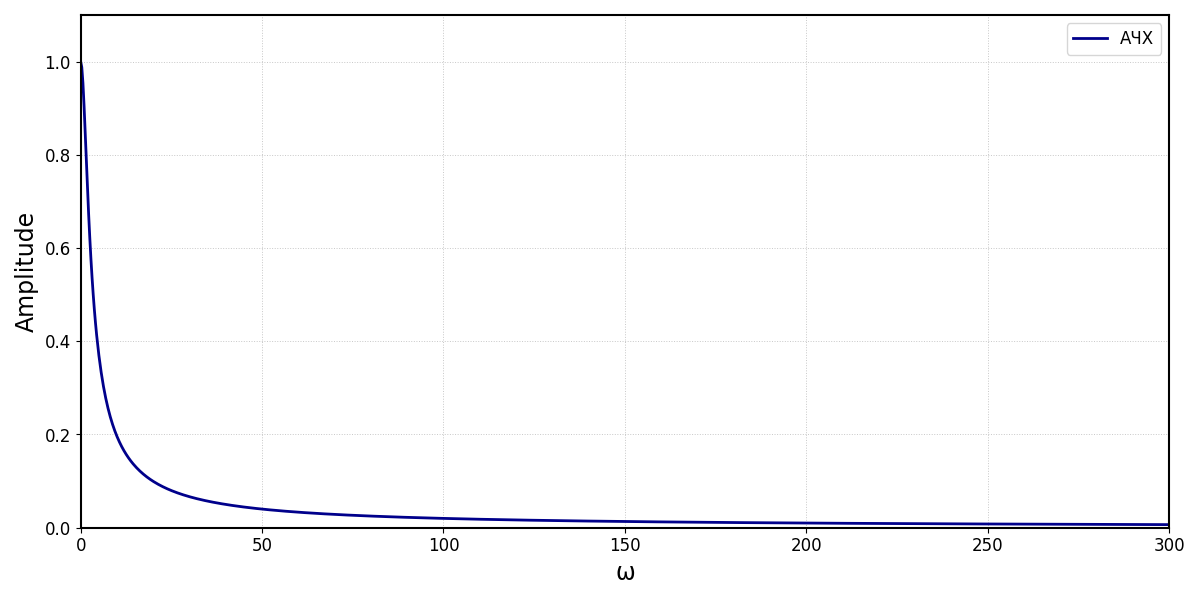
\includegraphics[width=1\textwidth]{../images/linearFilter/ACH0.5.png}
		\caption{График АЧХ. \(T = 0.5\)}  
		\label{fig:my_image}  
	\end{figure}
	
	\begin{figure}[H]  
		\centering
		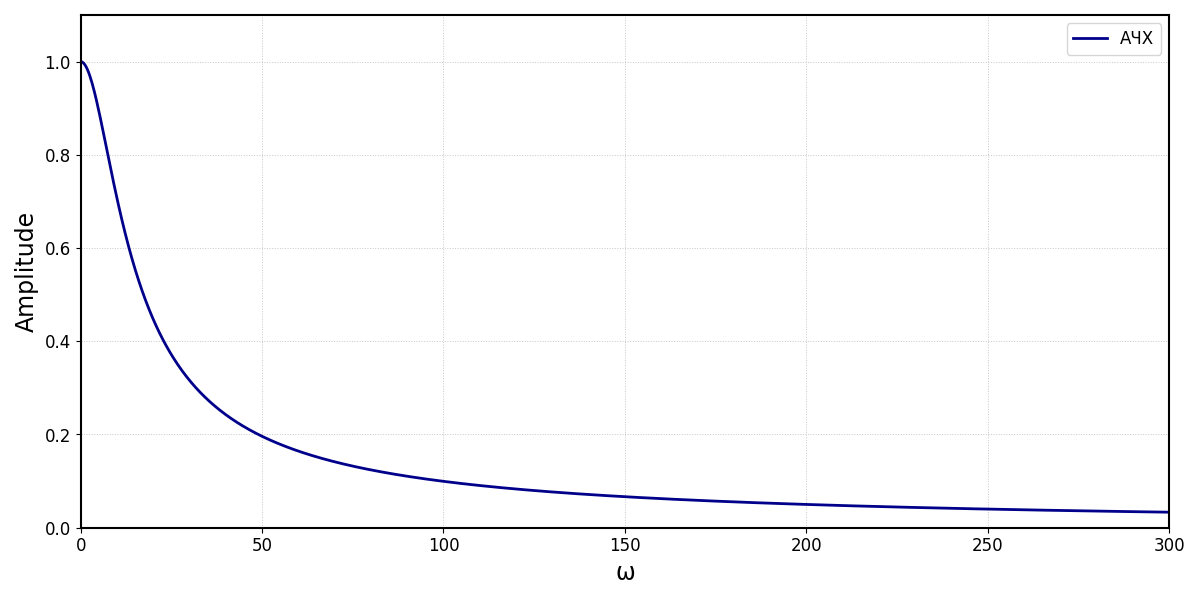
\includegraphics[width=1\textwidth]{../images/linearFilter/ACH0.1.png}
		\caption{График АЧХ. \(T = 0.1\)}  
		\label{fig:my_image}  
	\end{figure}
	
	
	\begin{figure}[H]  
		\centering
		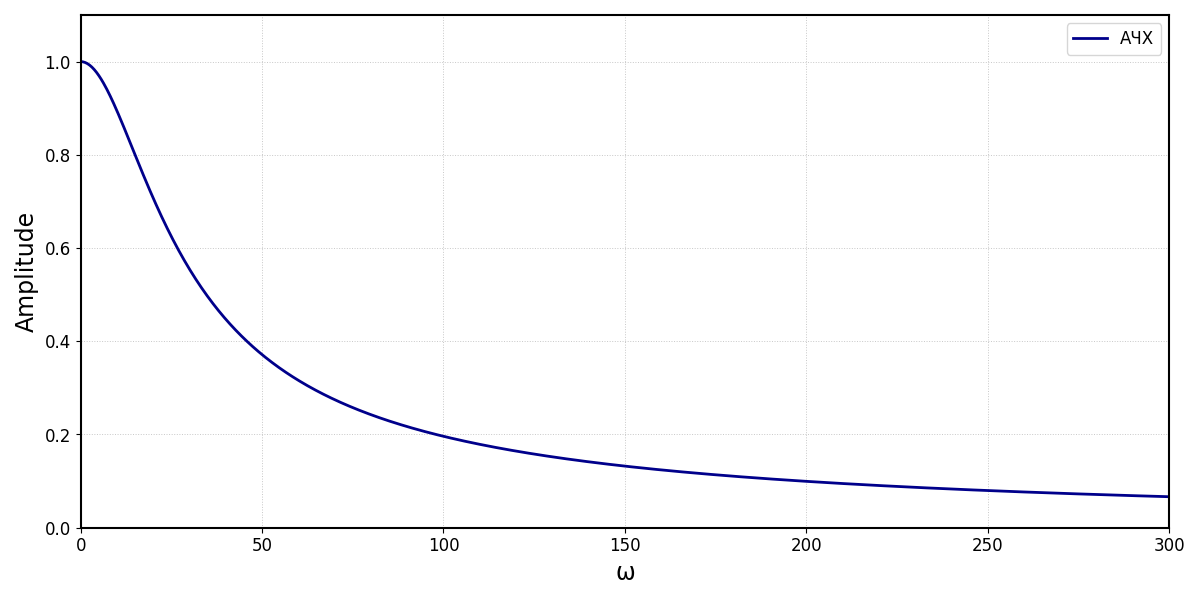
\includegraphics[width=1\textwidth]{../images/linearFilter/ACH0.05.png}
		\caption{График АЧХ. \(T = 0.05\)}  
		\label{fig:my_image}  
	\end{figure}
	
	\subsubsection{Графики сигналов}
	
	Зафиксирую срединное \(a = 4\) и буду менять параметр \(T\).
	
	\begin{figure}[H]  
		\centering
		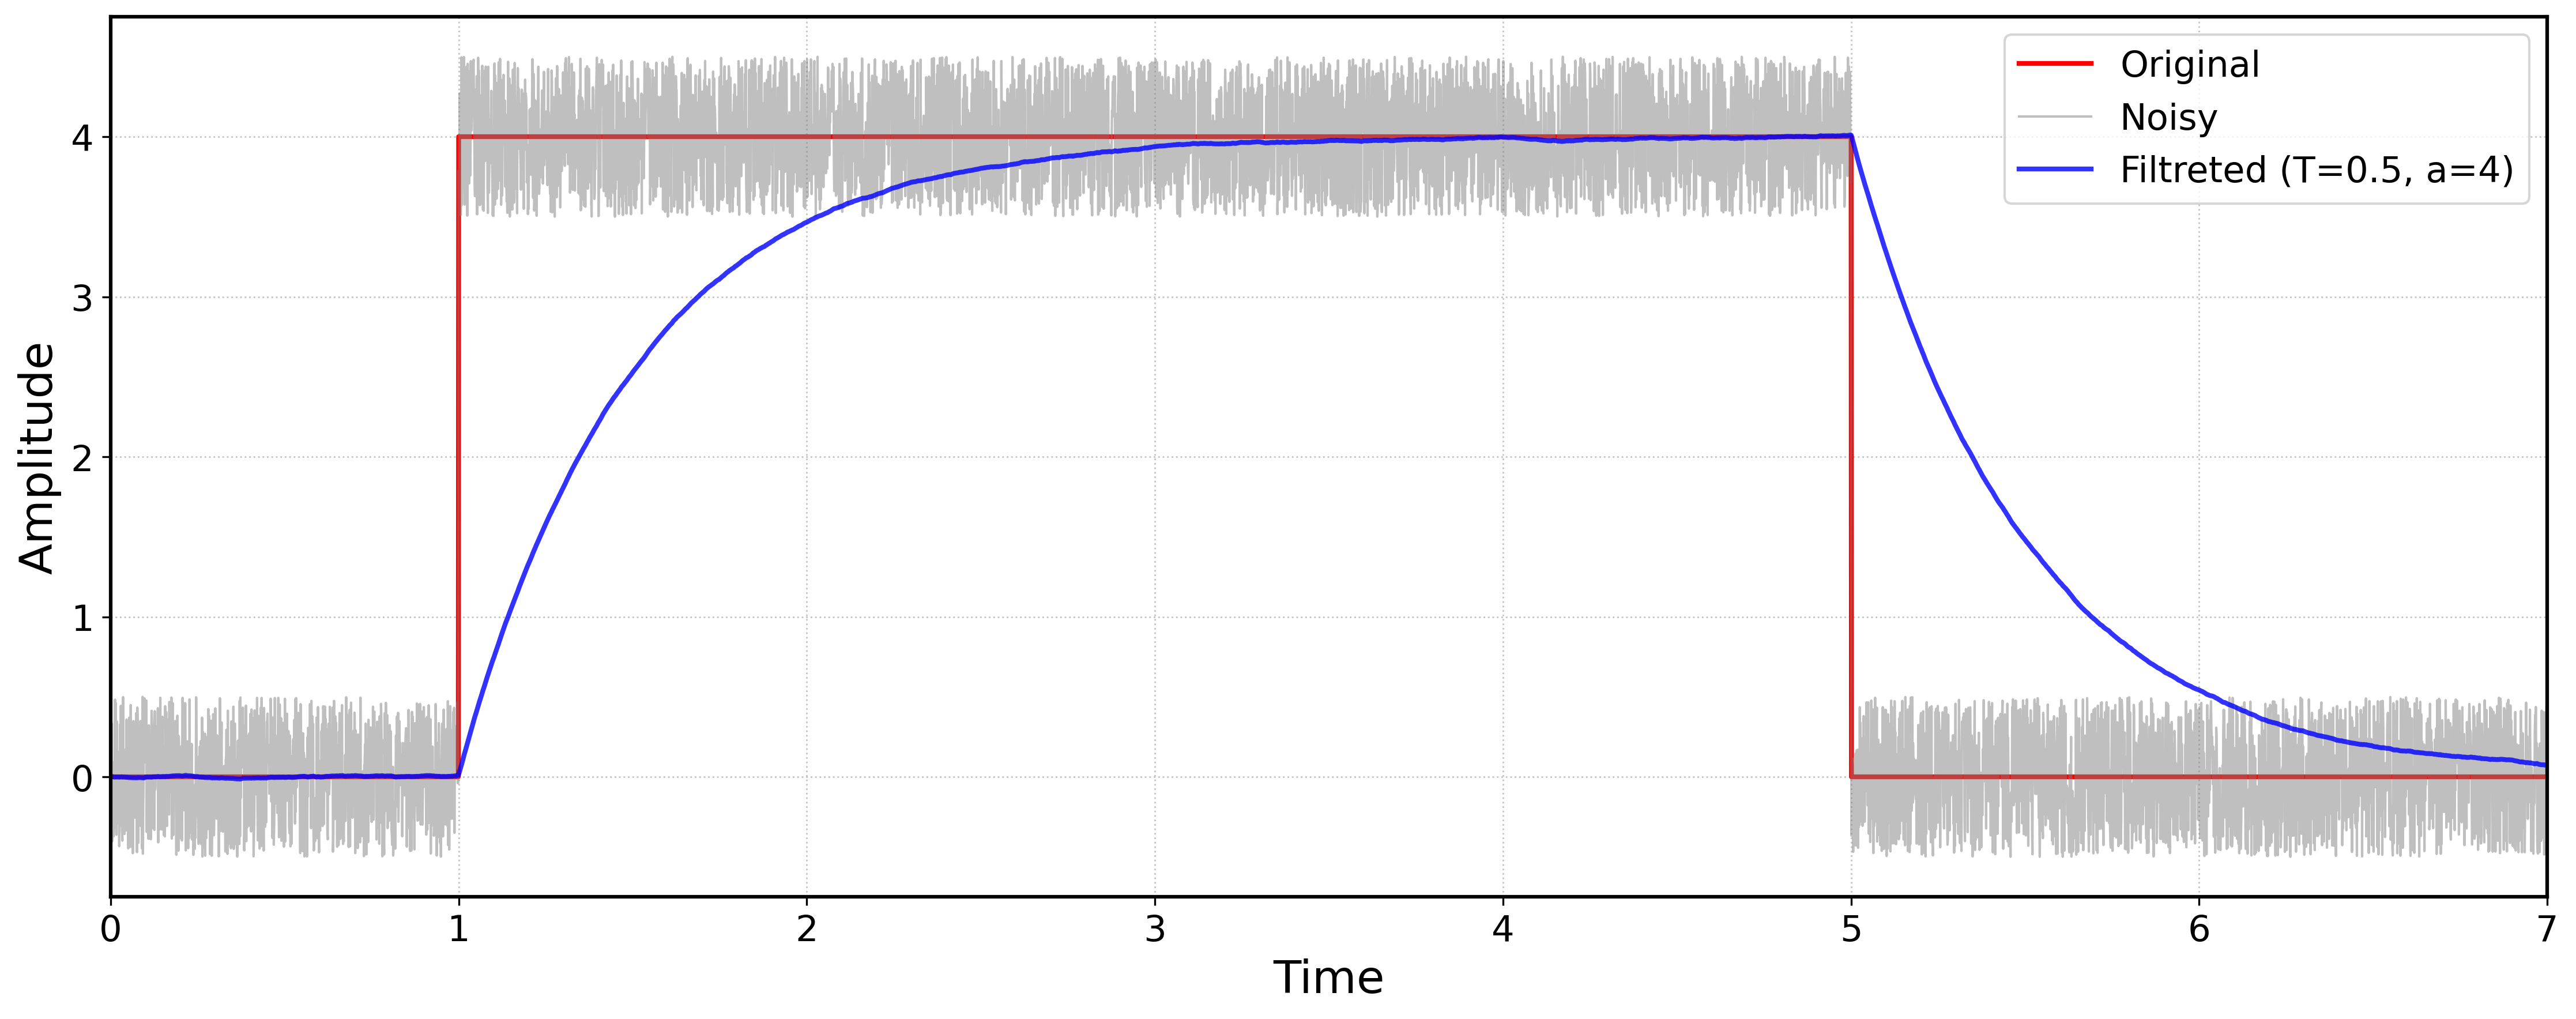
\includegraphics[width=1\textwidth]{../images/linearFilter/sig0.5.4.png}
		\caption{Сигналы. \(a = 4, T = 0.5\)}  
		\label{fig:my_image}  
	\end{figure}
	
	\begin{figure}[H]  
		\centering
		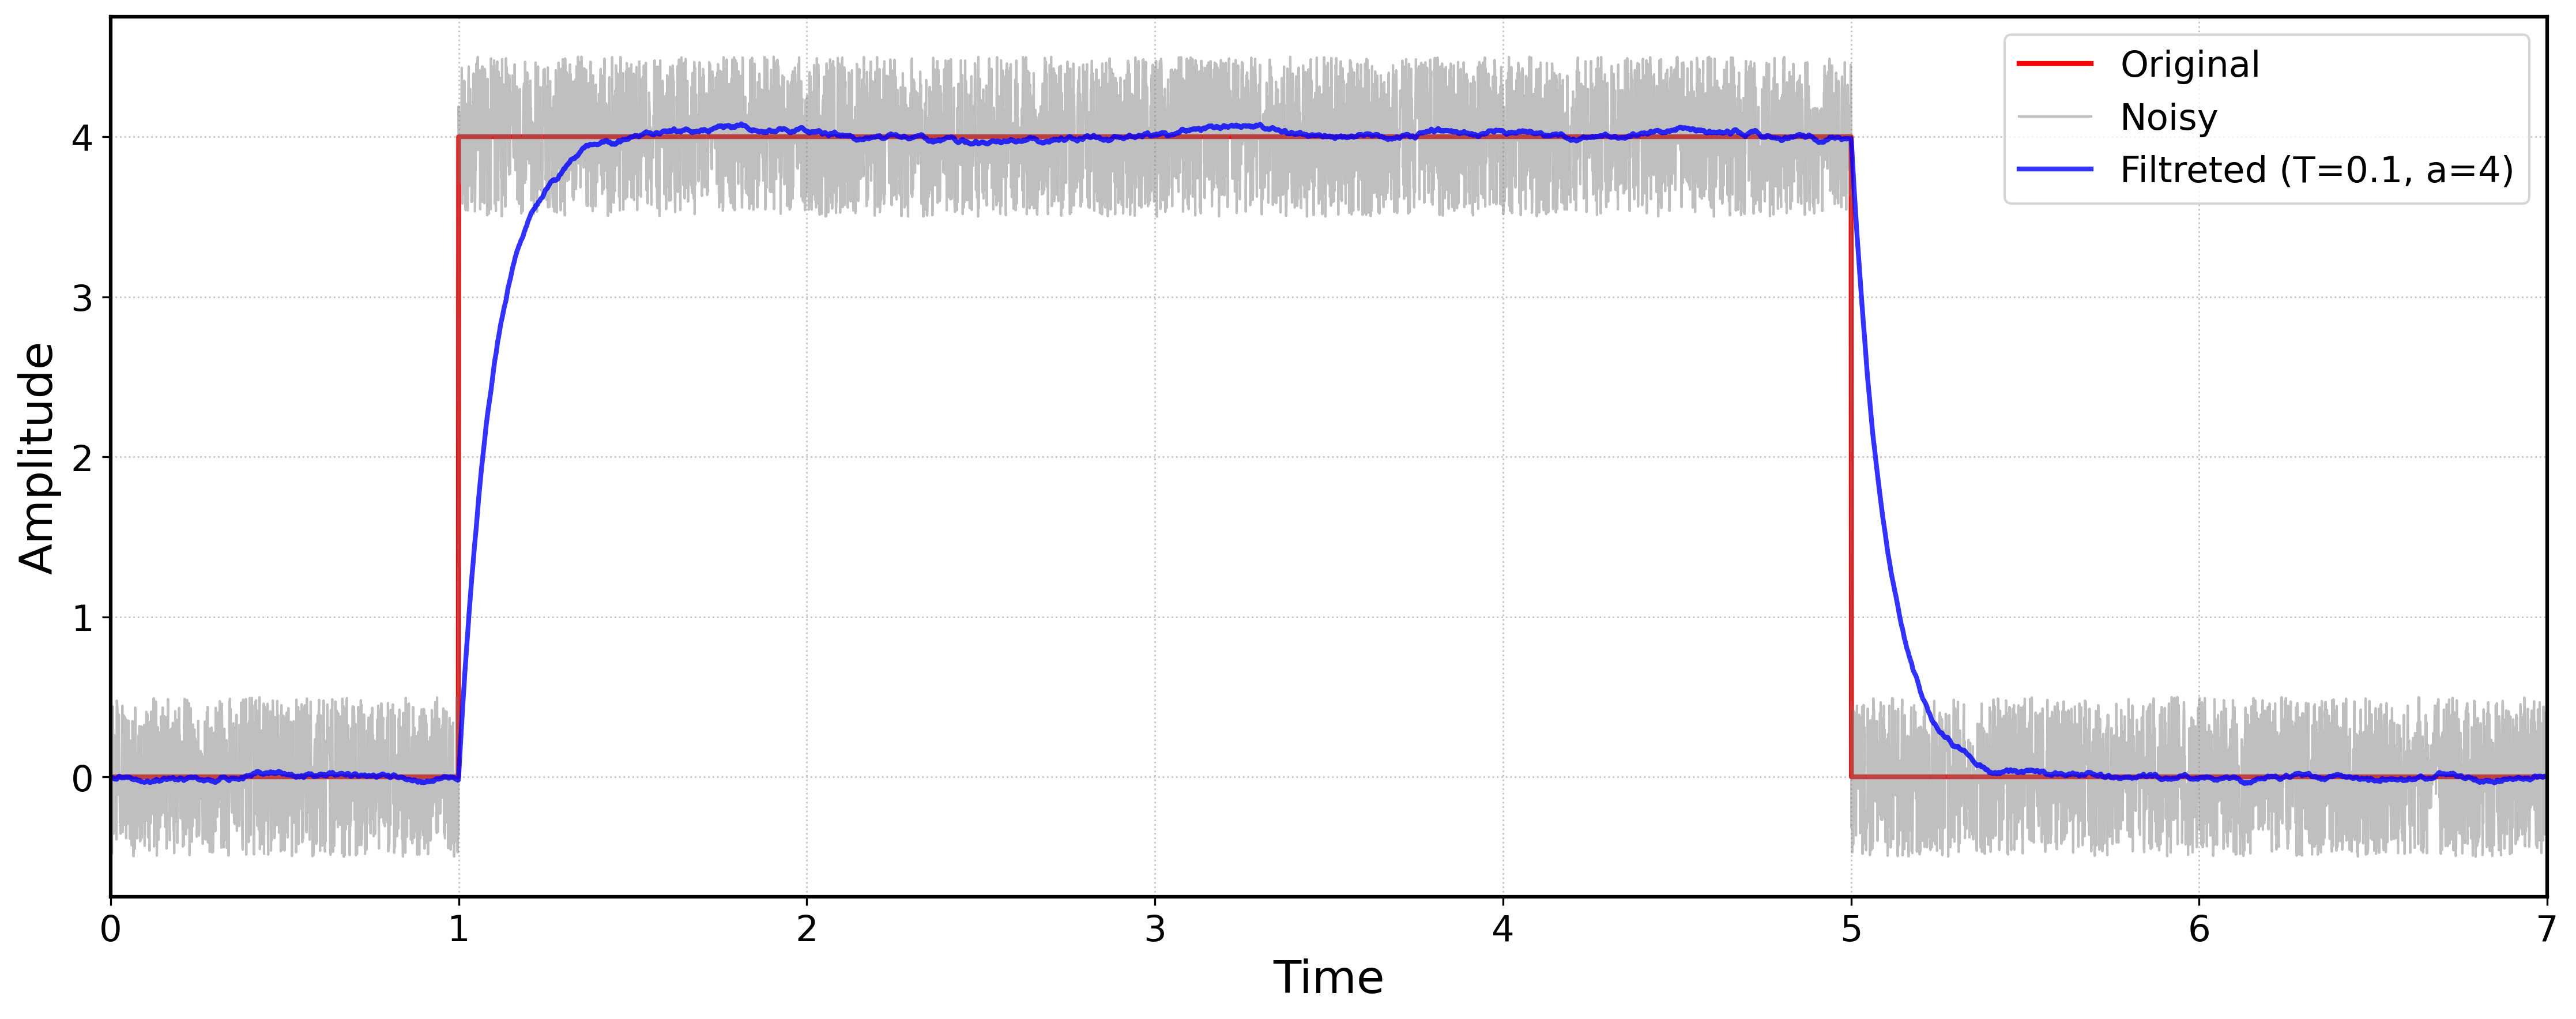
\includegraphics[width=1\textwidth]{../images/linearFilter/sig0.1.4.png}
		\caption{Сигналы. \(a = 4, T = 0.1\)}  
		\label{fig:my_image}  
	\end{figure}
	
	\begin{figure}[H]  
		\centering
		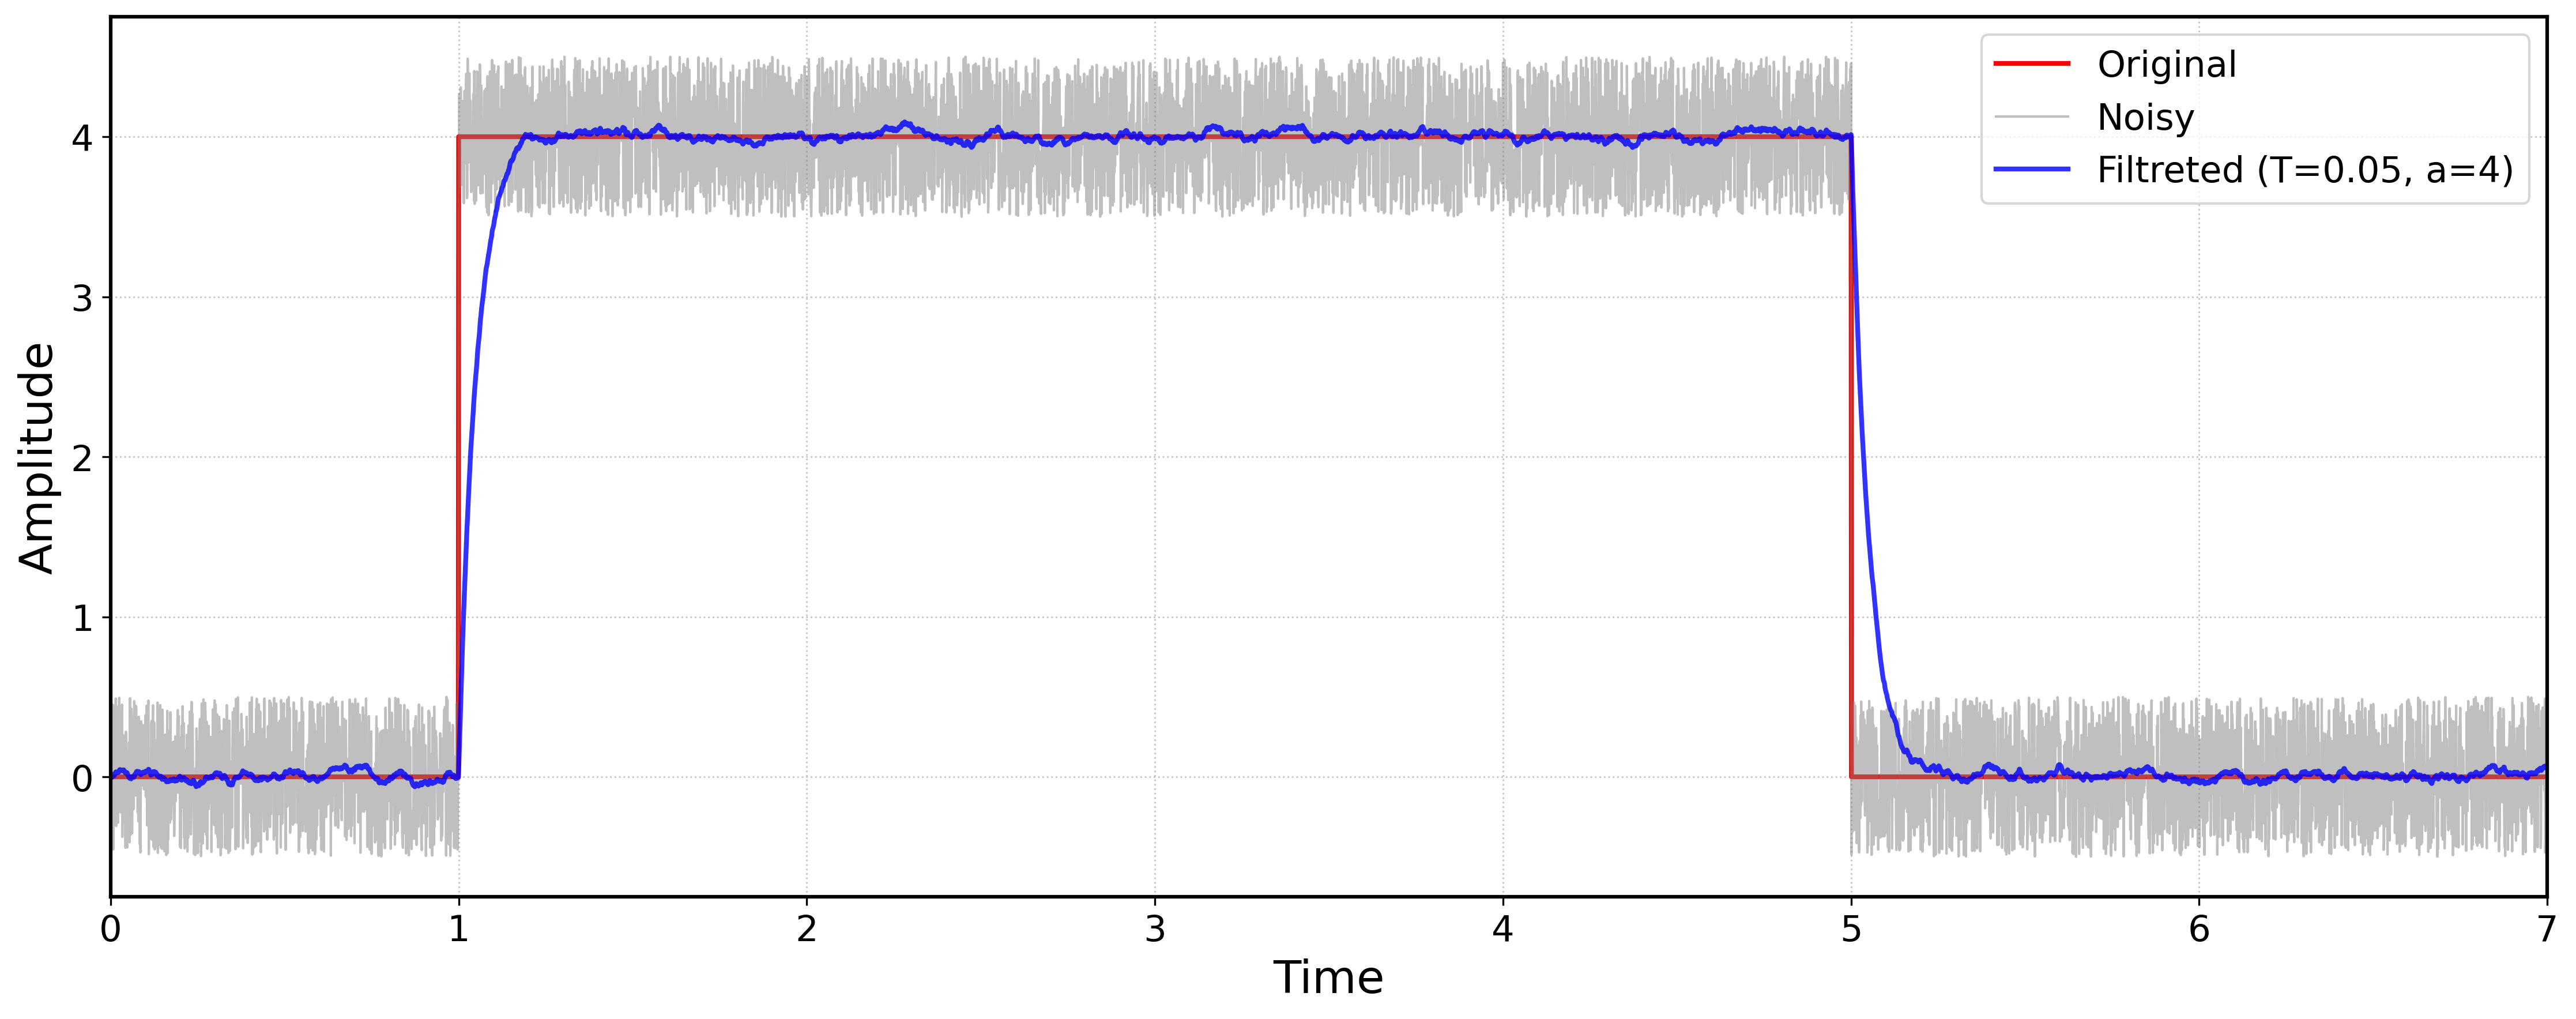
\includegraphics[width=1\textwidth]{../images/linearFilter/sig0.05.4.png}
		\caption{Сигналы. \(a = 4, T = 0.05\)}  
		\label{fig:my_image}  
	\end{figure}
	
	Зафиксирую срединное значение \(T = 0.1\) и буду менять параметр \(a\).
	
	\begin{figure}[H]  
		\centering
		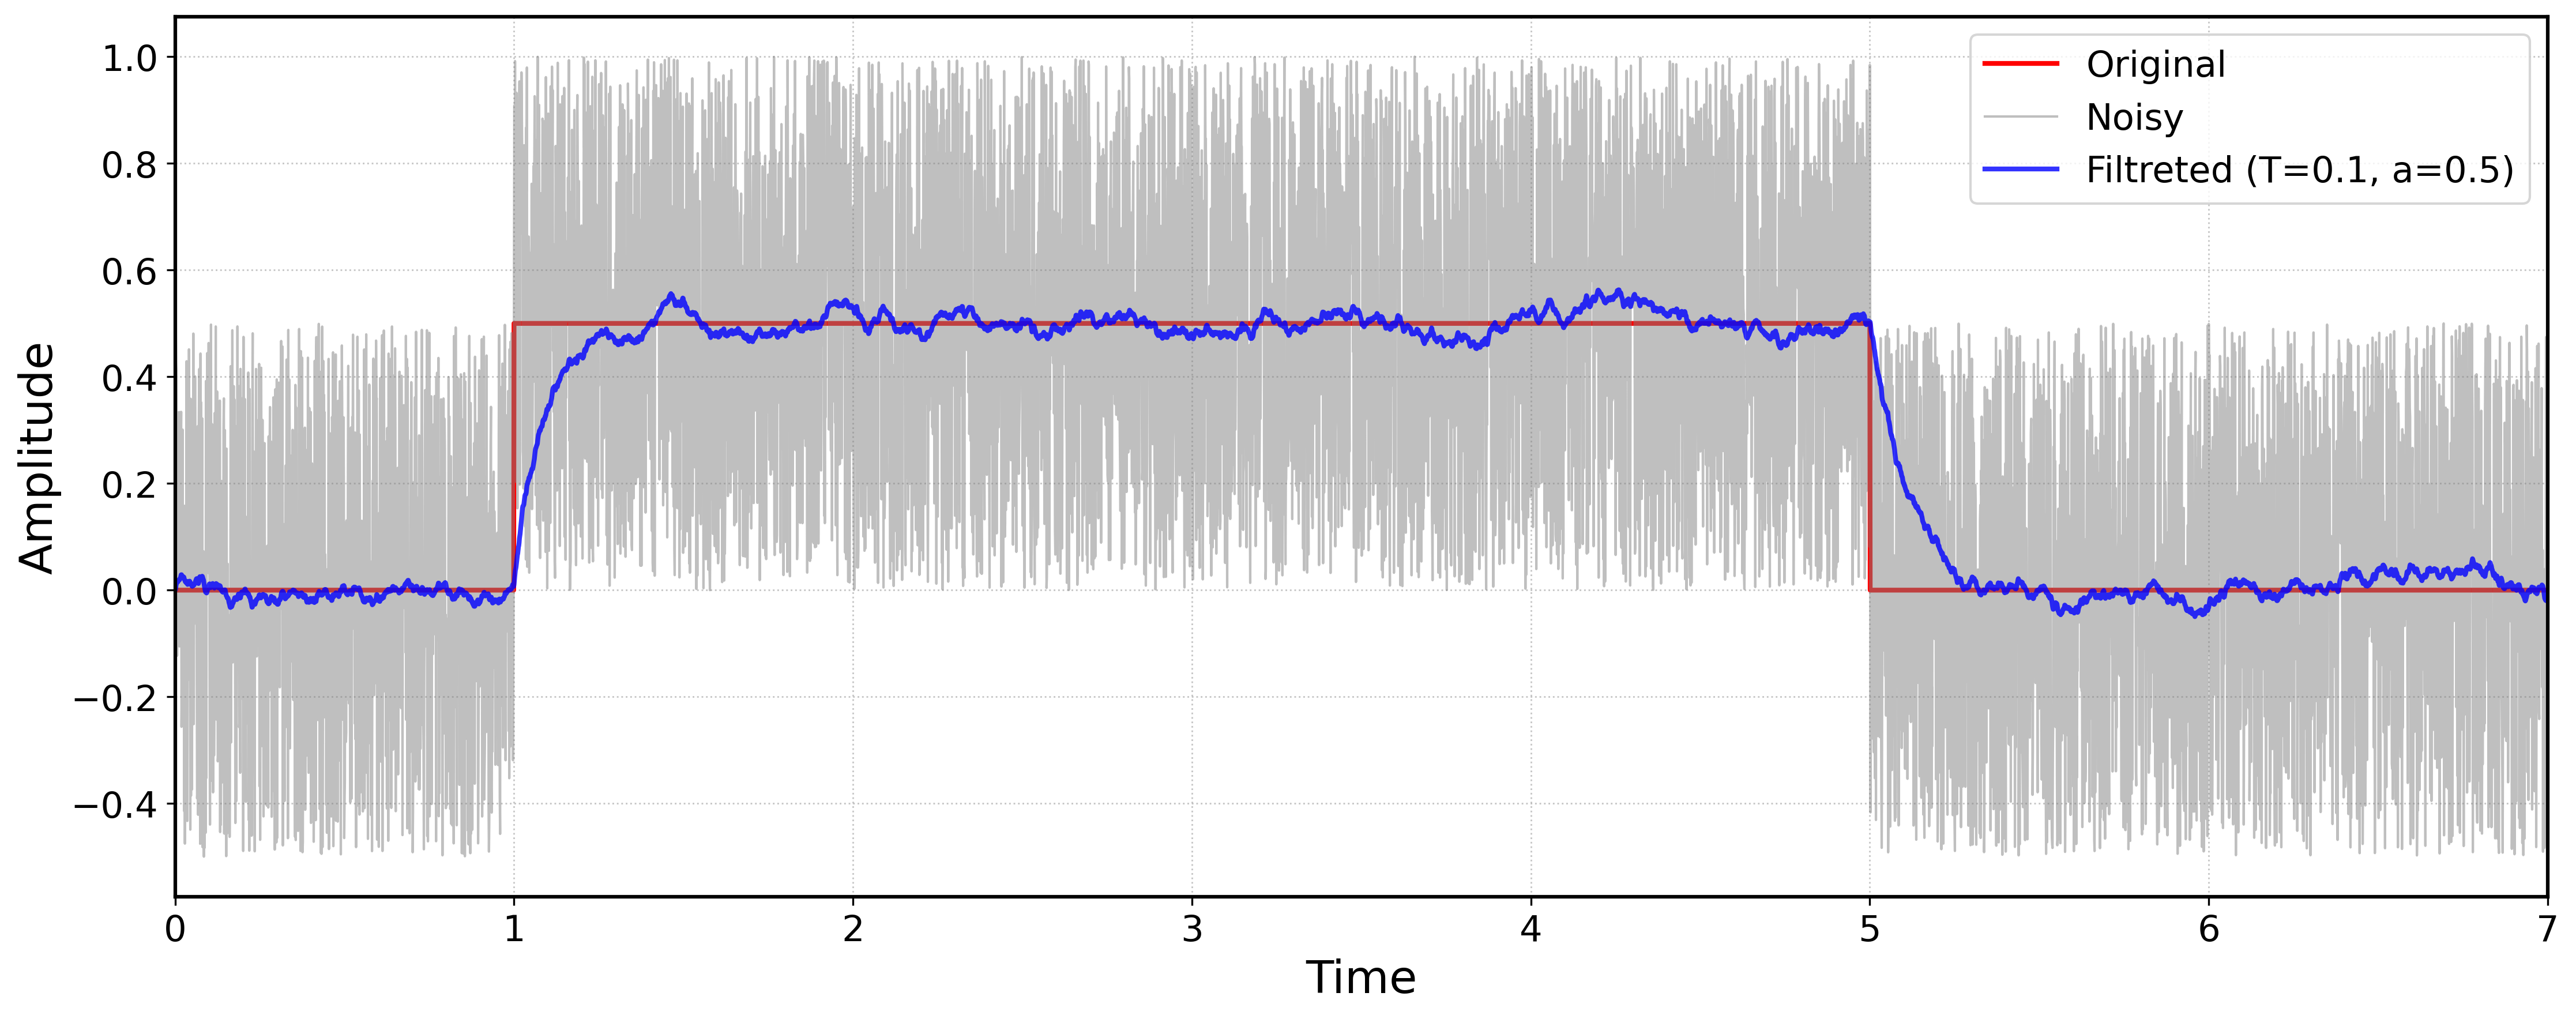
\includegraphics[width=1\textwidth]{../images/linearFilter/sig0.1.0.5.png}
		\caption{Сигналы. \(a = 0.5, T = 0.1\)}  
		\label{fig:my_image}  
	\end{figure}
	
	\begin{figure}[H]  
		\centering
		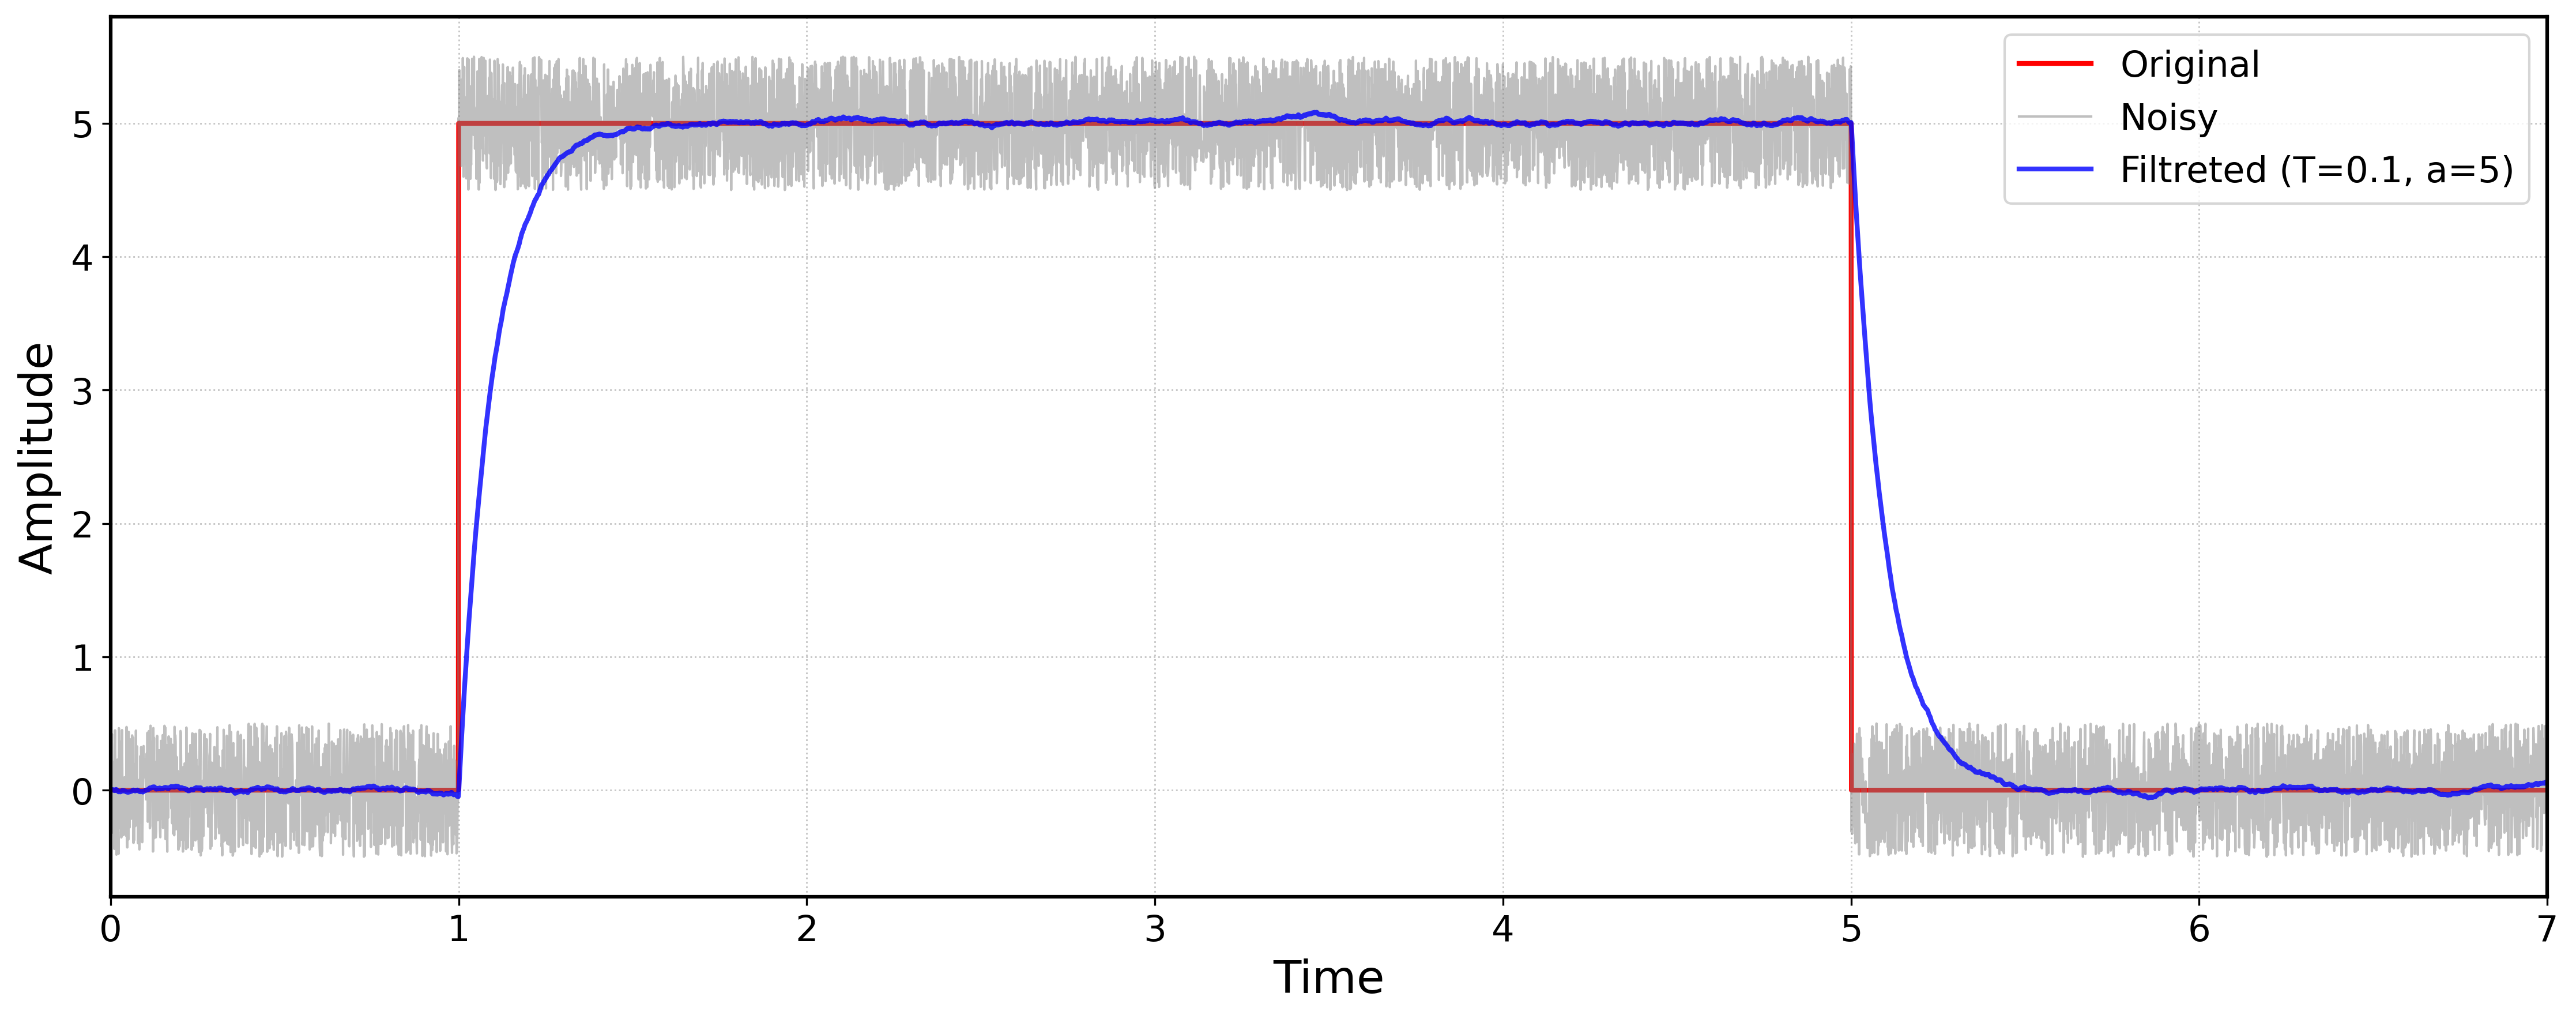
\includegraphics[width=1\textwidth]{../images/linearFilter/sig0.1.5.png}
		\caption{Сигналы. \(a = 5, T = 0.1\)}  
		\label{fig:my_image}  
	\end{figure}
	
	\begin{figure}[H]  
		\centering
		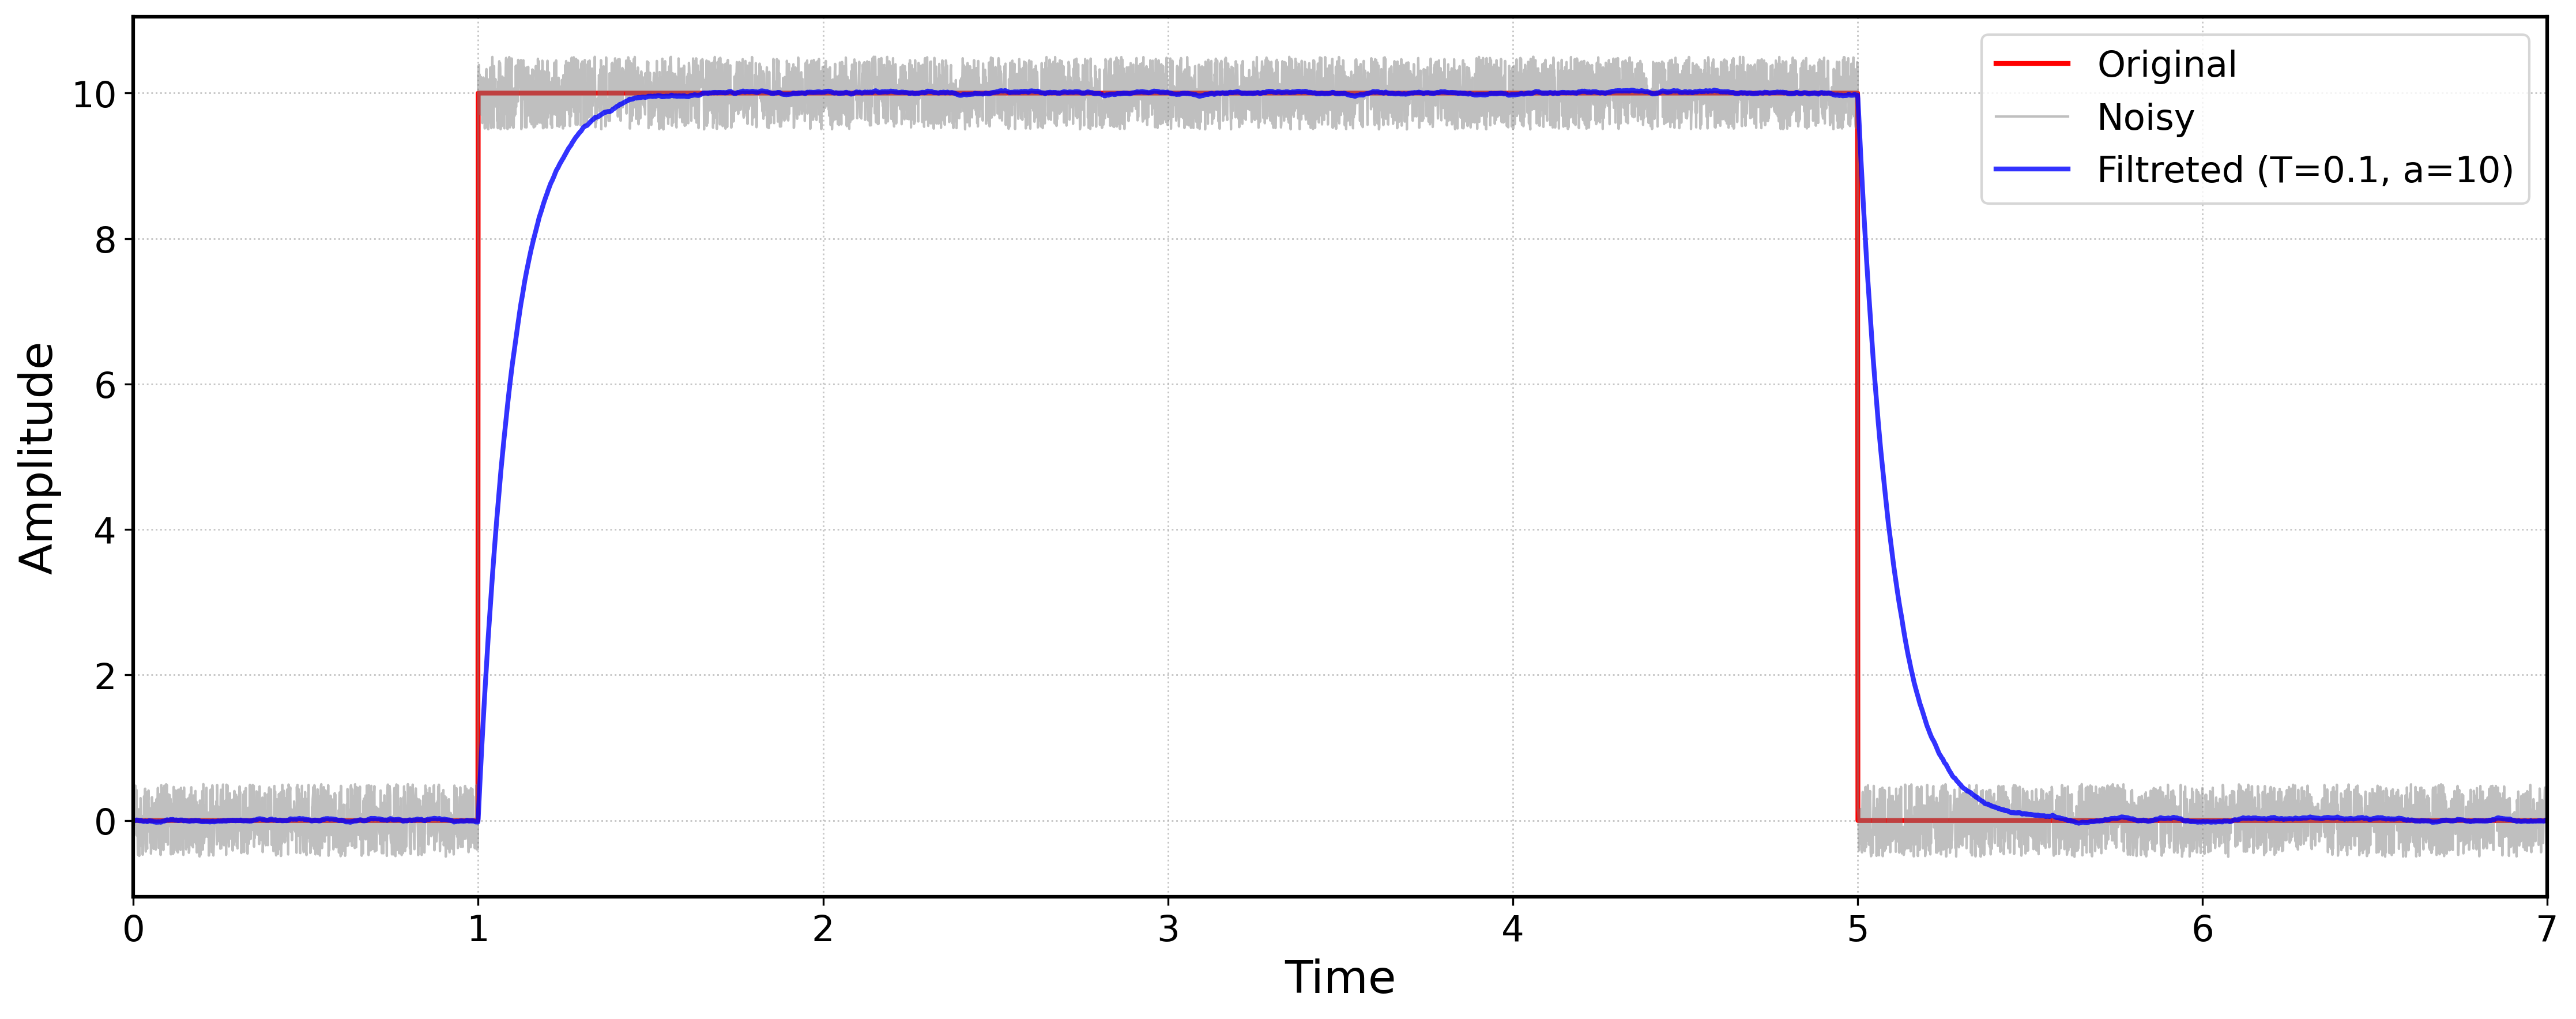
\includegraphics[width=1\textwidth]{../images/linearFilter/sig0.1.10.png}
		\caption{Сигналы. \(a = 10, T = 0.1\)}  
		\label{fig:my_image}  
	\end{figure}
	
	\subsubsection{Сравнение временной и частотной фильтрации}
	
	Построю сравнительные графики сигналов: фильтрованного и полученного после обратного преобразования Фурье произведения частотной передаточной функции фильтра и образа зашумленного \(W_1(i\omega)\cdot \hat{u}(\omega)\).\\
	
	
	Зафиксирую параметр \(a = 4\) и буду менять параметр \(T\)
	\begin{figure}[H]  
		\centering
		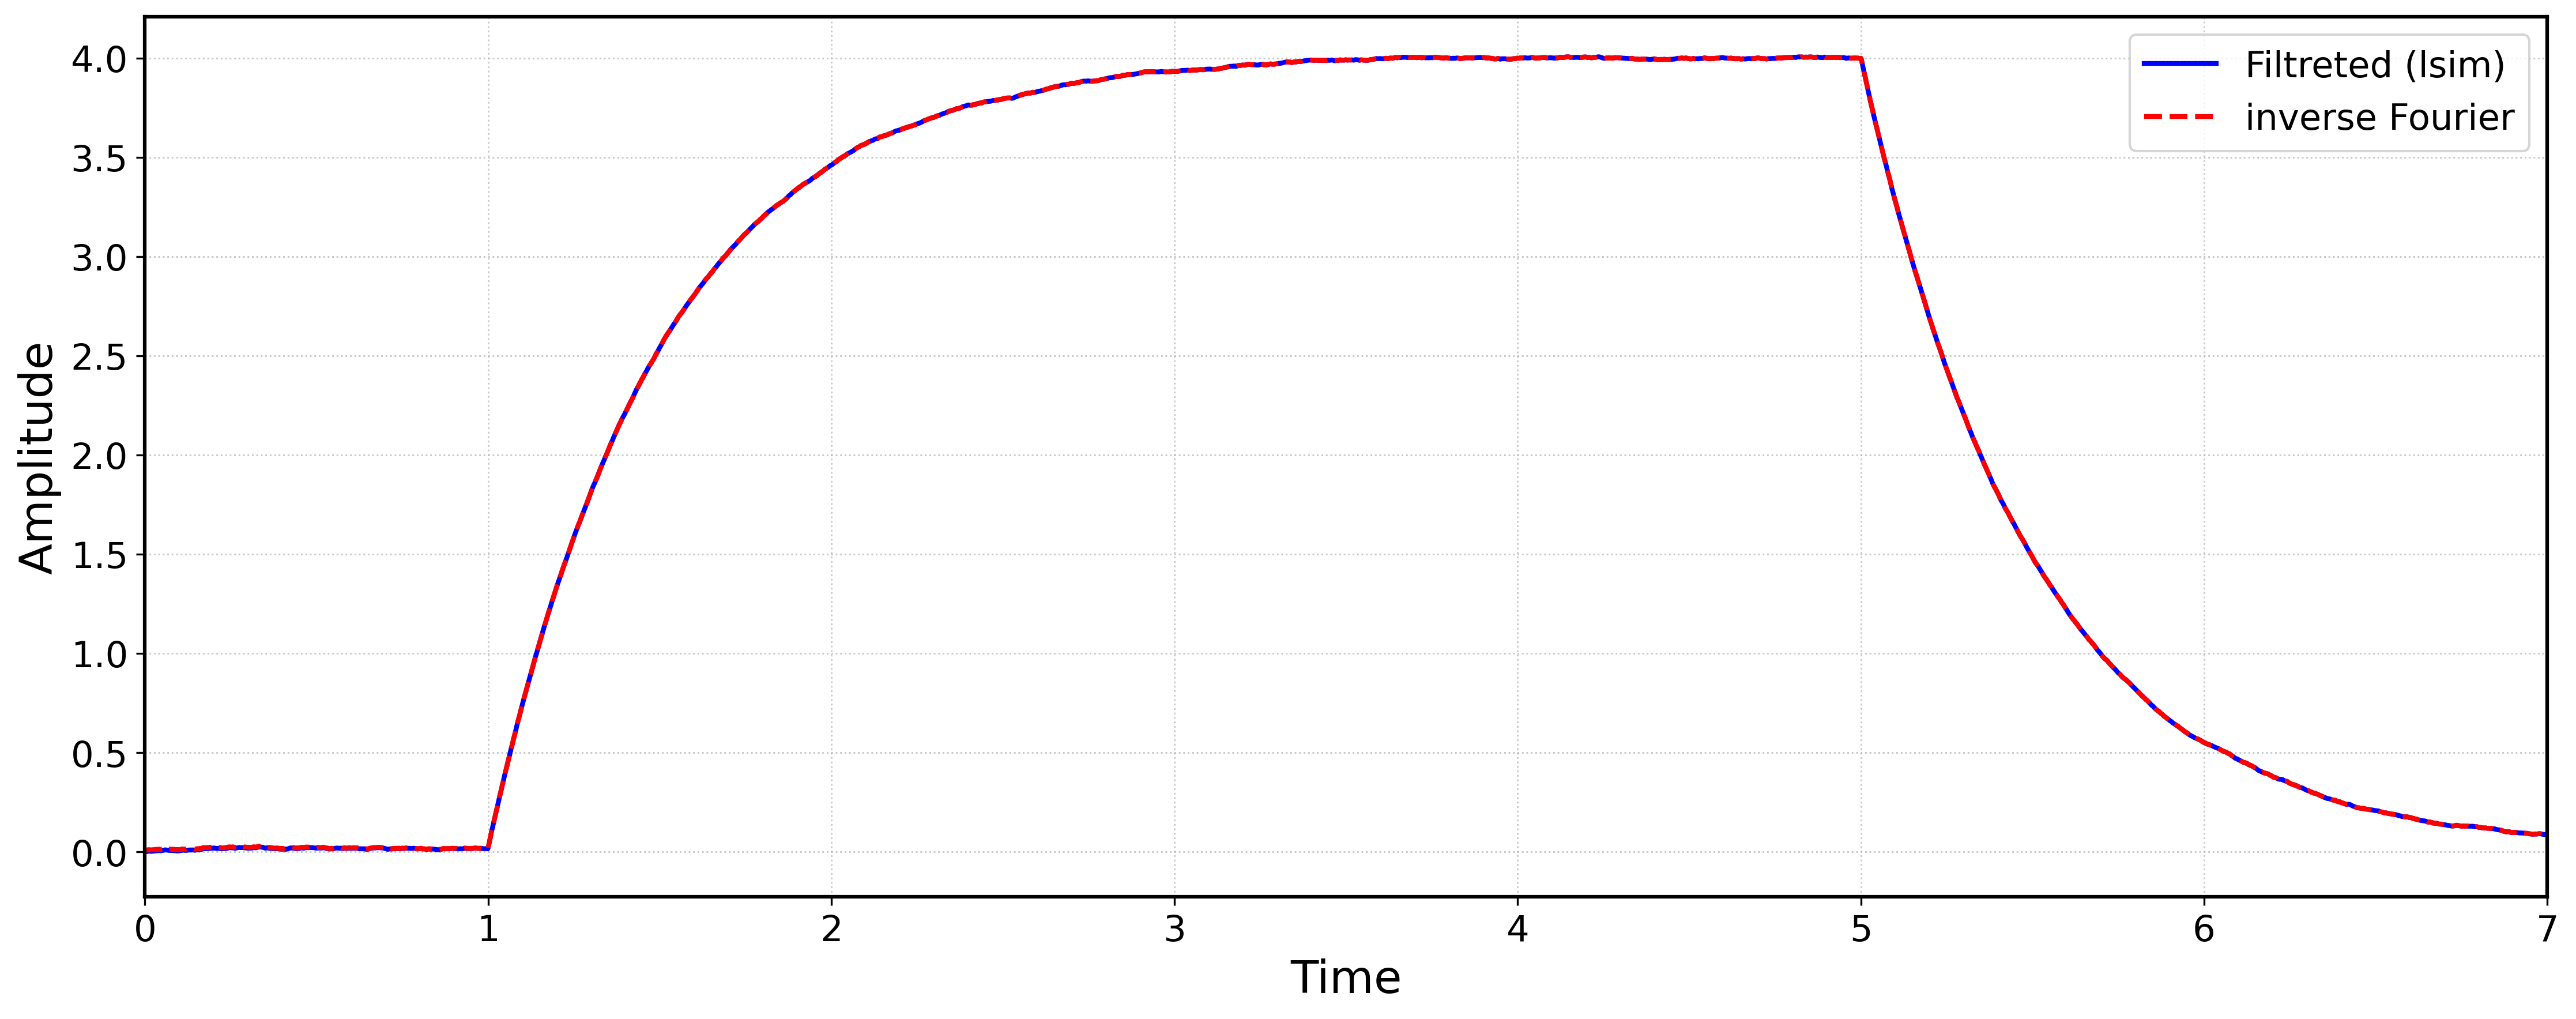
\includegraphics[width=1\textwidth]{../images/linearFilter/3.4.0.5.png}
		\caption{Сравнение методов фильтрации. \(a = 4, T = 0.5\)}  
		\label{fig:my_image}  
	\end{figure}
	
	\begin{figure}[H]  
		\centering
		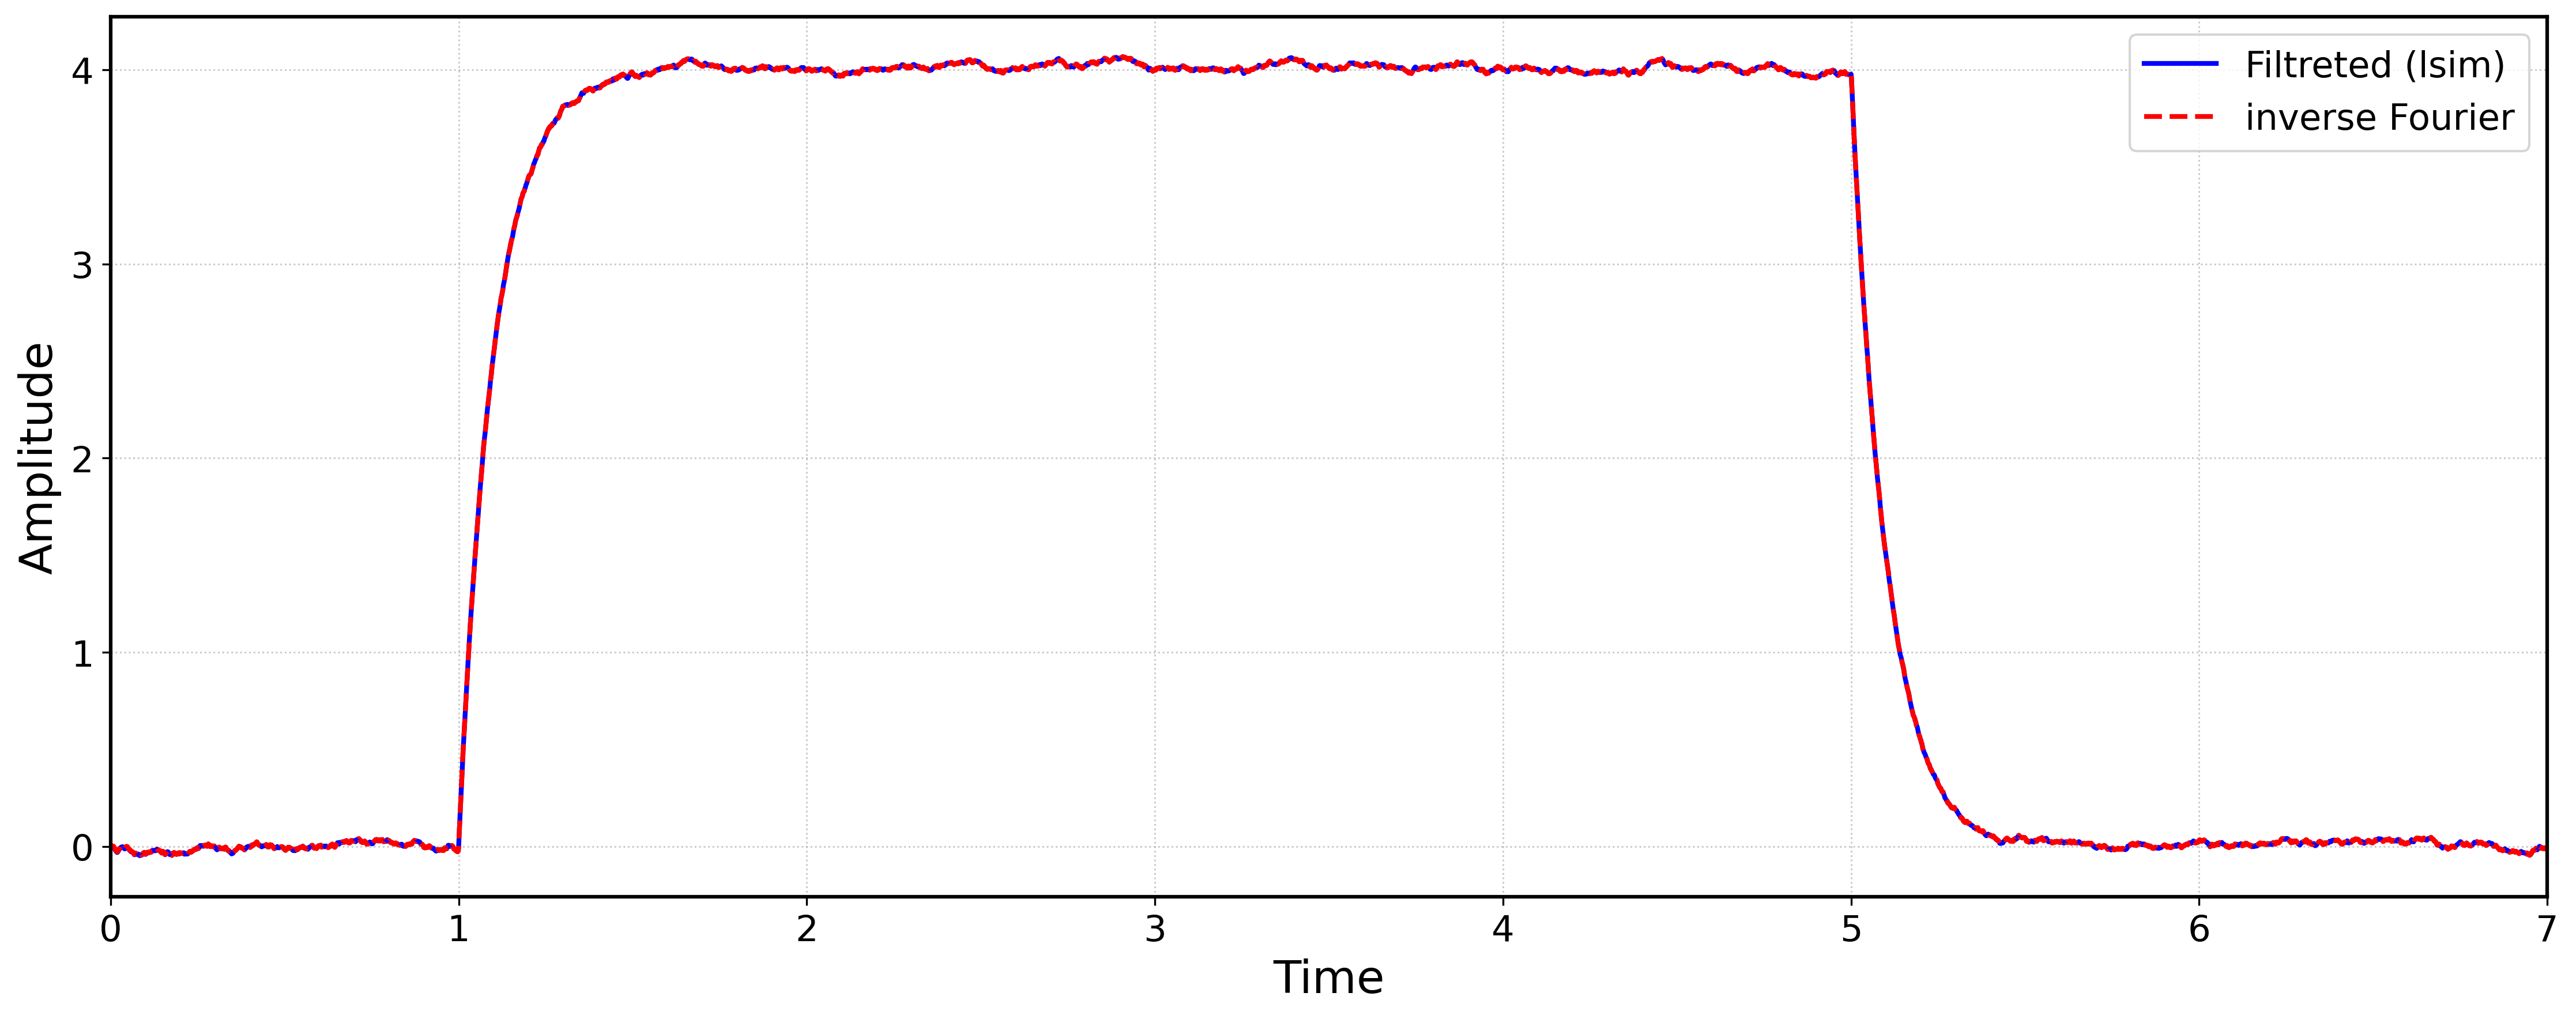
\includegraphics[width=1\textwidth]{../images/linearFilter/3.4.0.1.png}
		\caption{Сравнение методов фильтрации. \(a = 4, T = 0.1\)}  
		\label{fig:my_image}  
	\end{figure}
	
	\begin{figure}[H]  
		\centering
		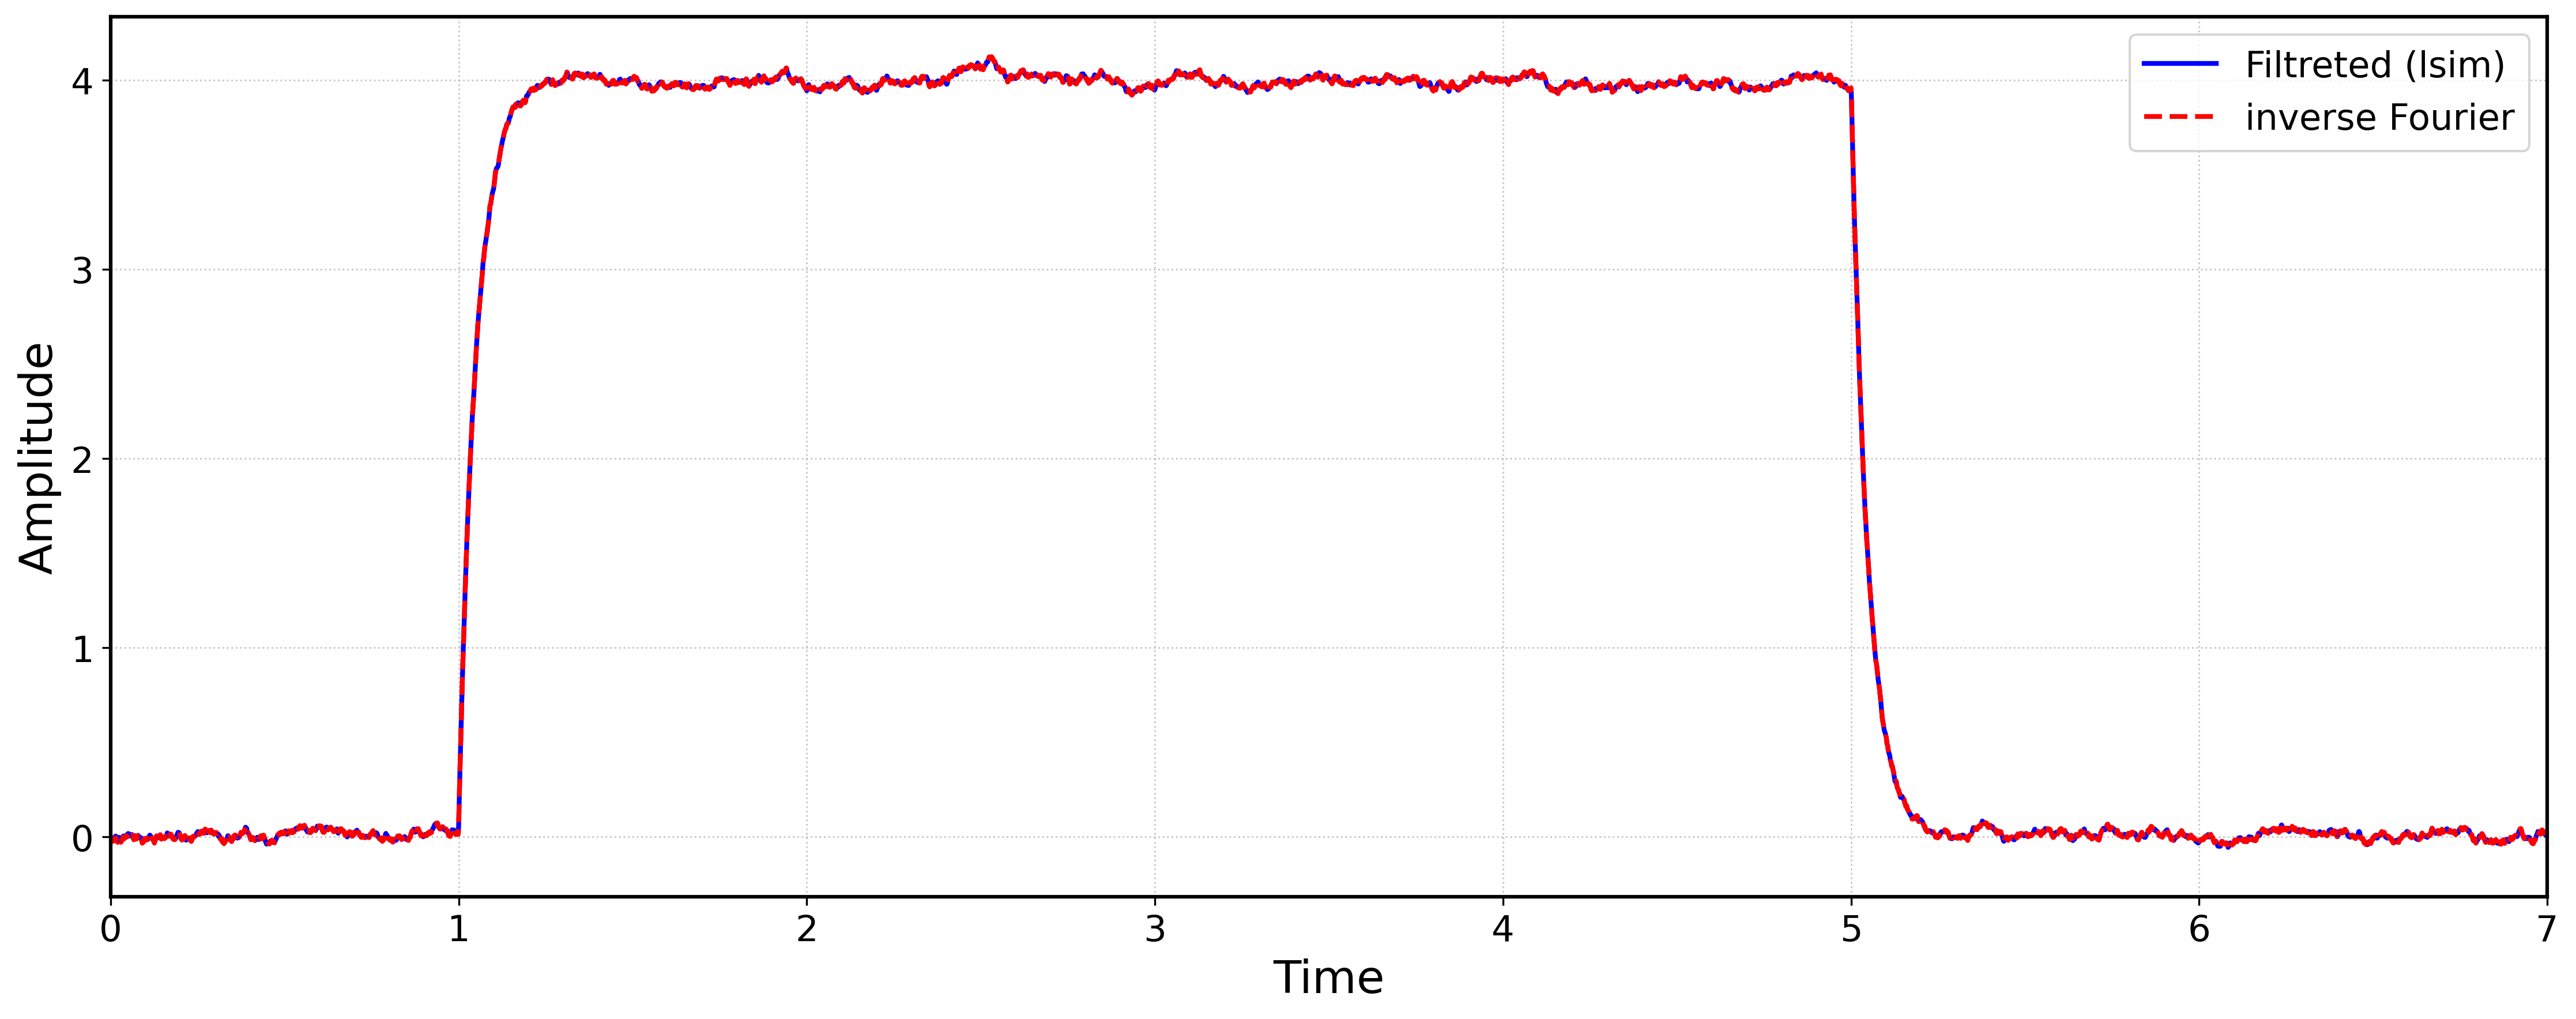
\includegraphics[width=1\textwidth]{../images/linearFilter/3.4.0.05.png}
		\caption{Сравнение методов фильтрации. \(a = 4, T = 0.05\)}  
		\label{fig:my_image}  
	\end{figure}
	
	Зафиксирую параметр \(T = 0.1\) и буду менять параметр \(a\)
	
	\begin{figure}[H]  
		\centering
		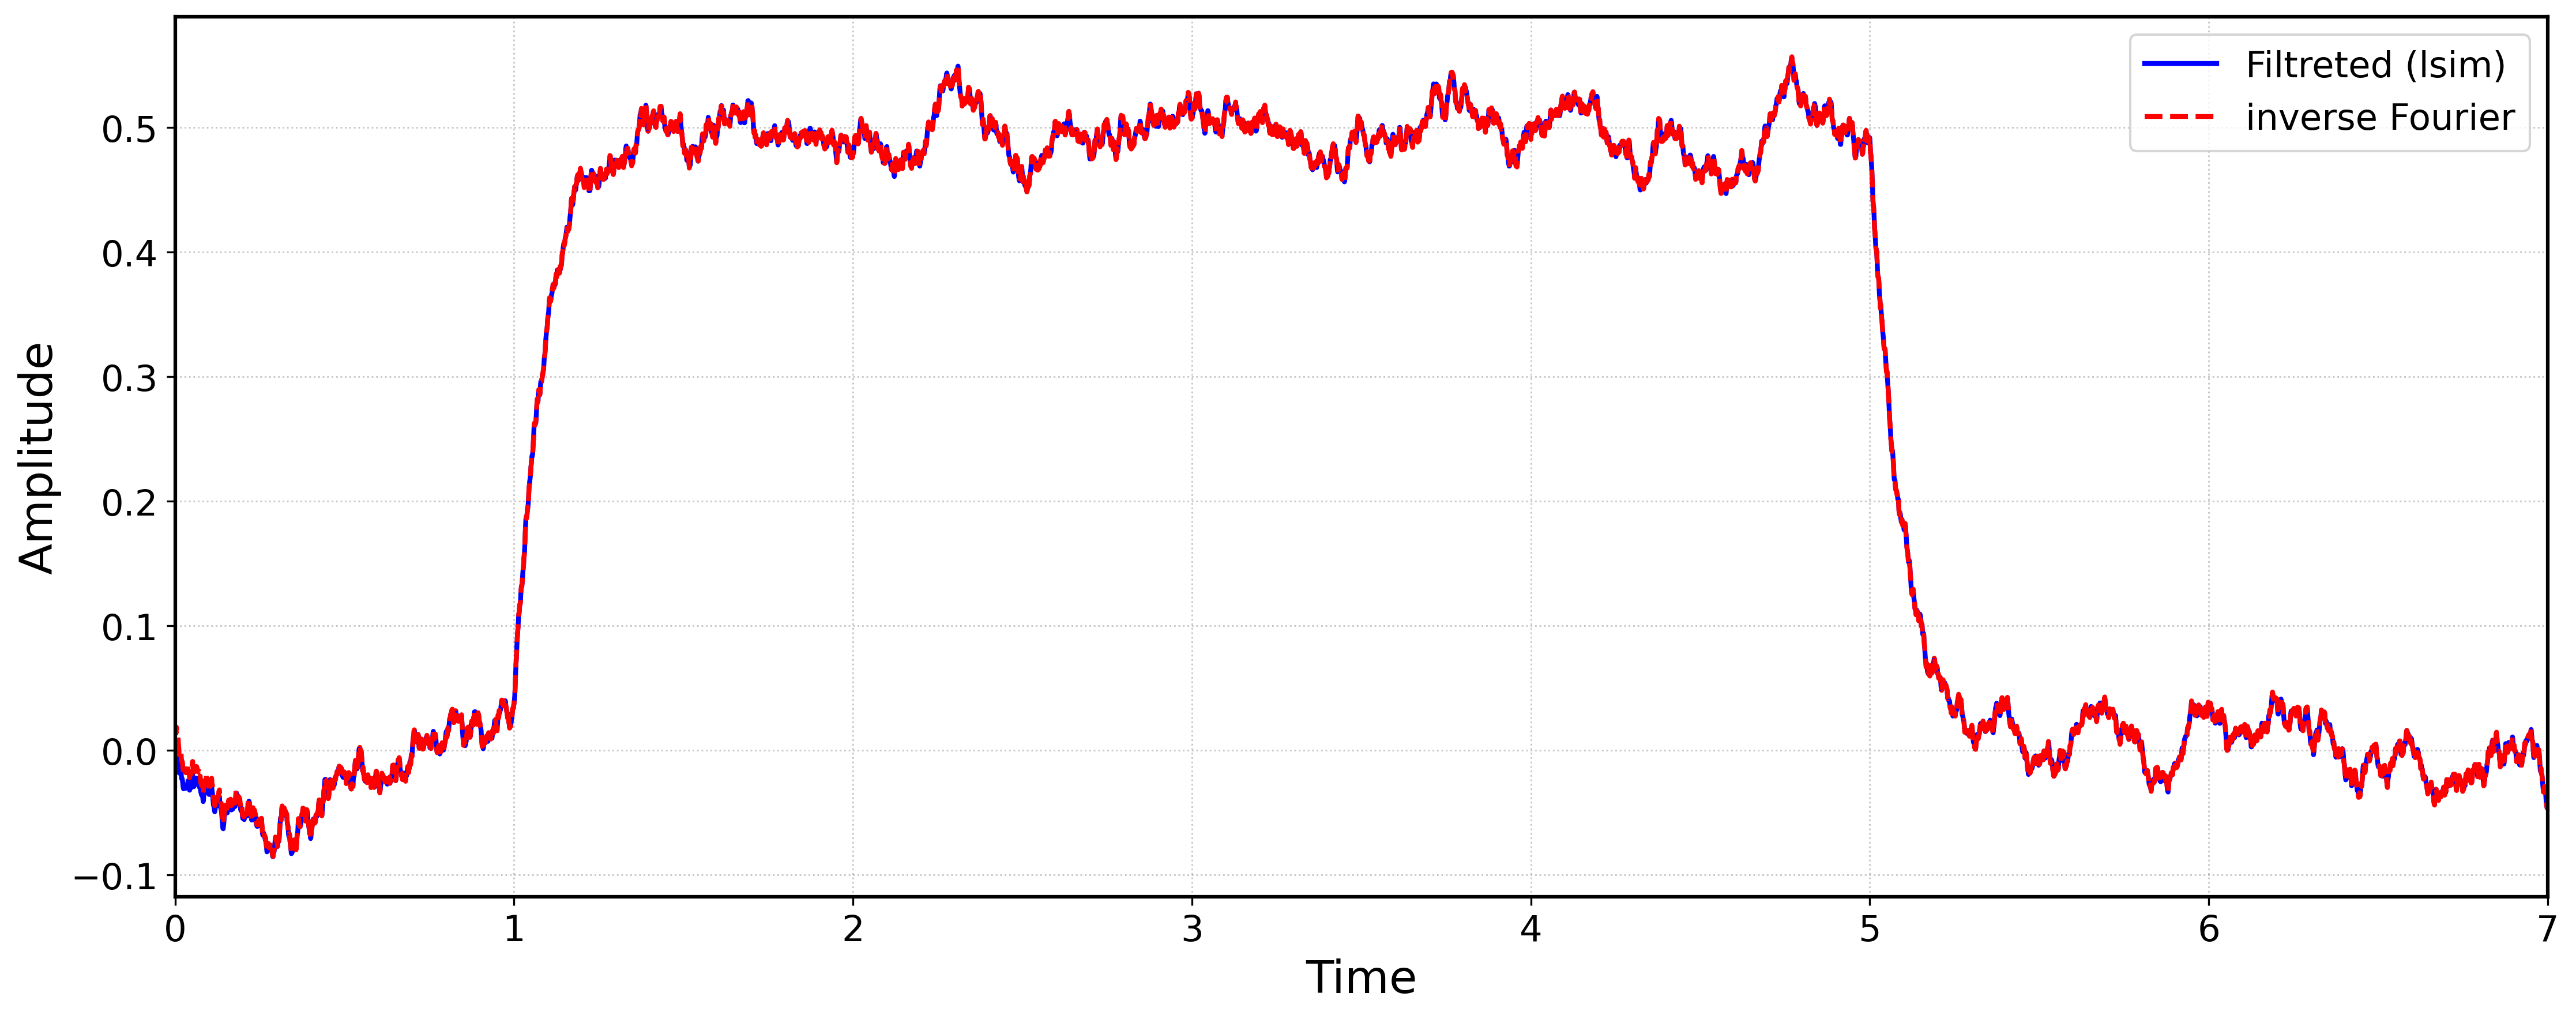
\includegraphics[width=1\textwidth]{../images/linearFilter/3.0.5.0.1.png}
		\caption{Сравнение методов фильтрации. \(a = 0.5, T = 0.1\)}  
		\label{fig:my_image}  
	\end{figure}
	
	\begin{figure}[H]  
		\centering
		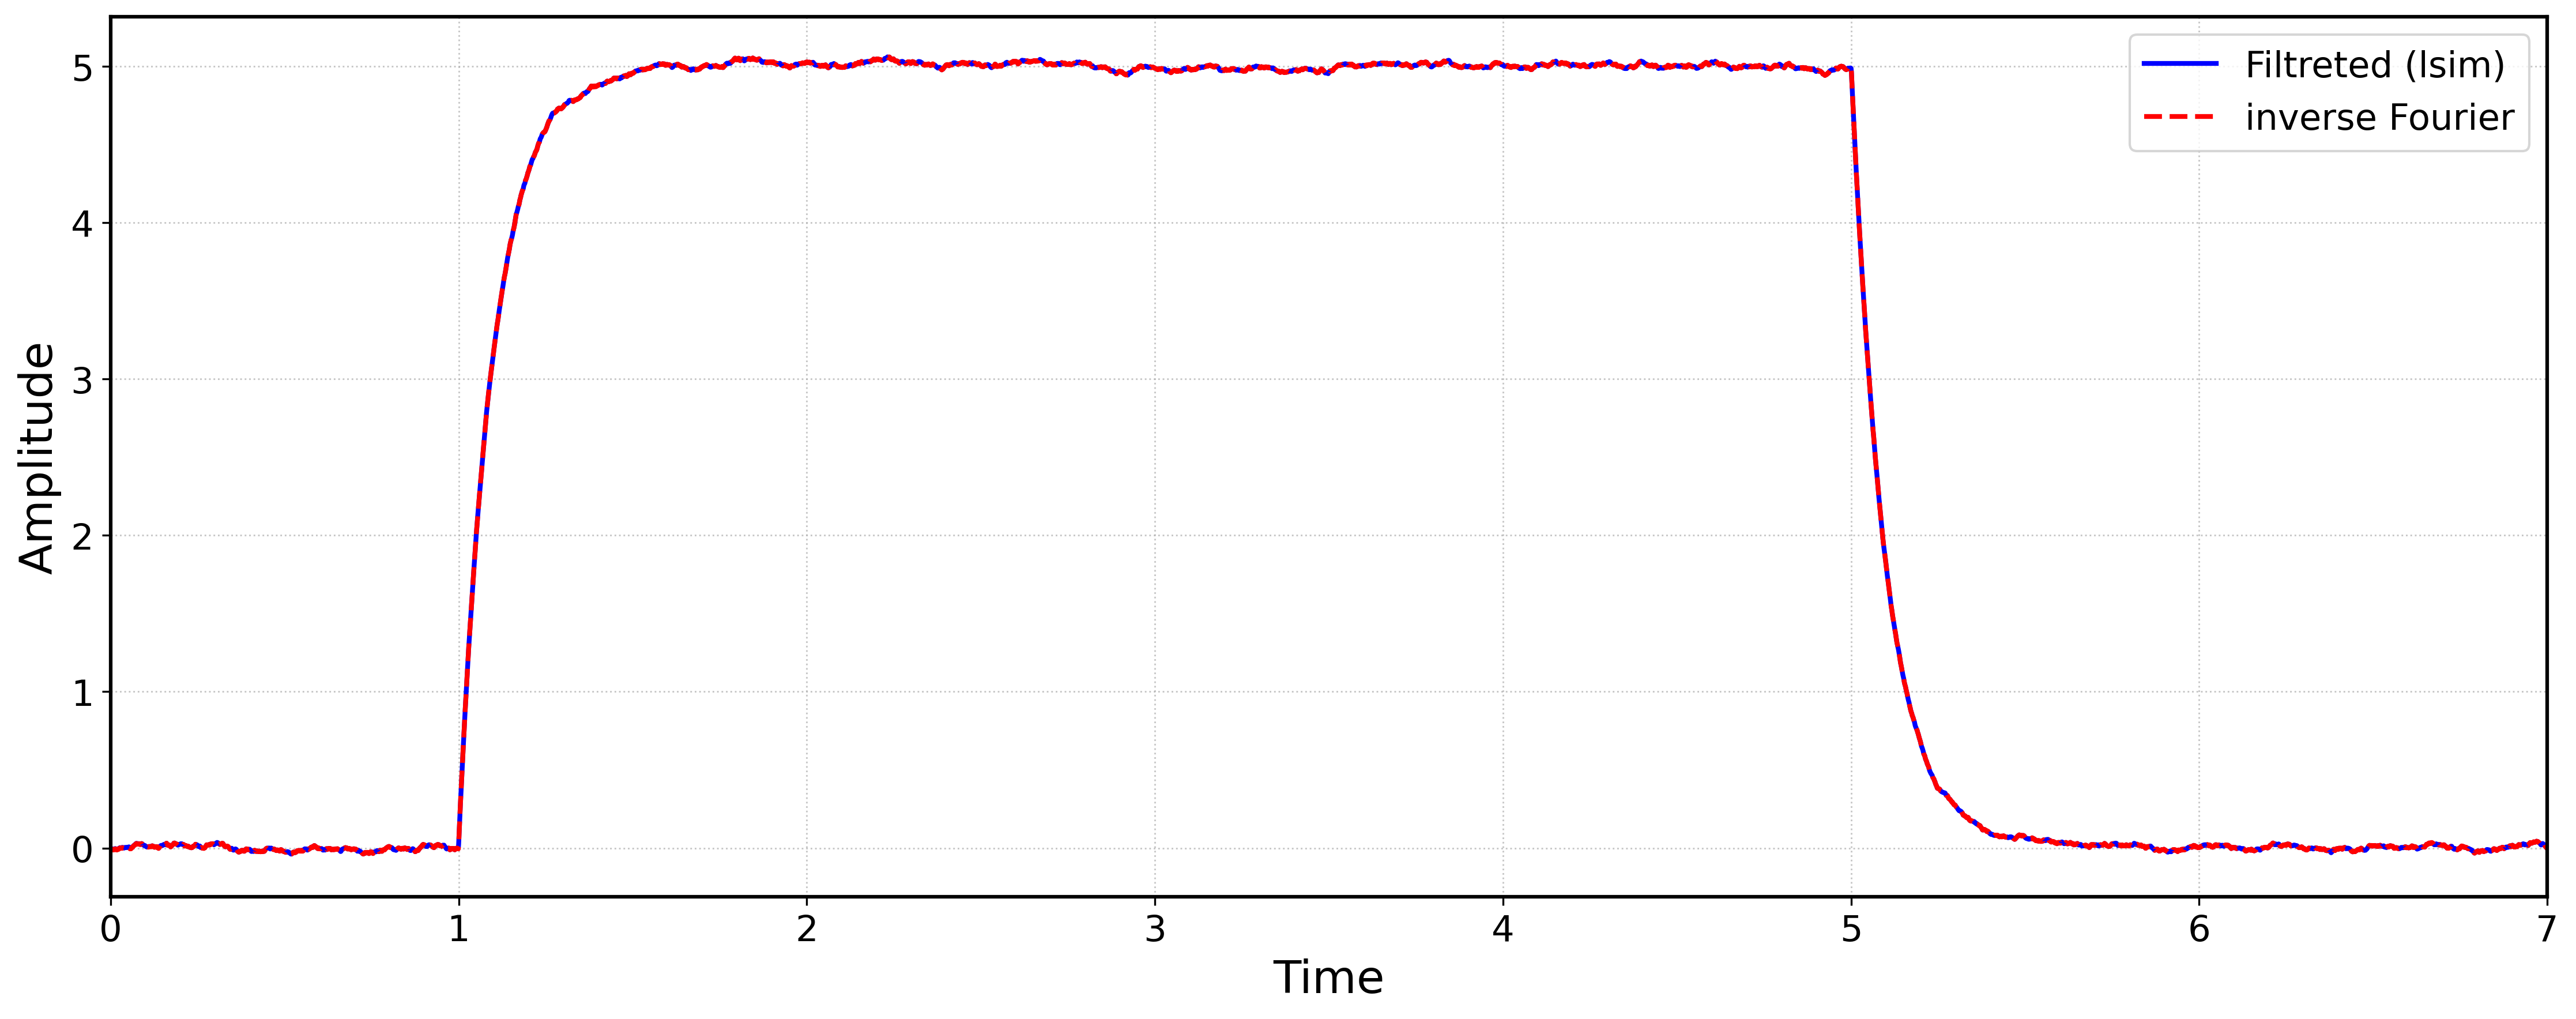
\includegraphics[width=1\textwidth]{../images/linearFilter/3.5.0.1.png}
		\caption{Сравнение методов фильтрации. \(a = 5, T = 0.1\)}  
		\label{fig:my_image}  
	\end{figure}
	
	\begin{figure}[H]  
		\centering
		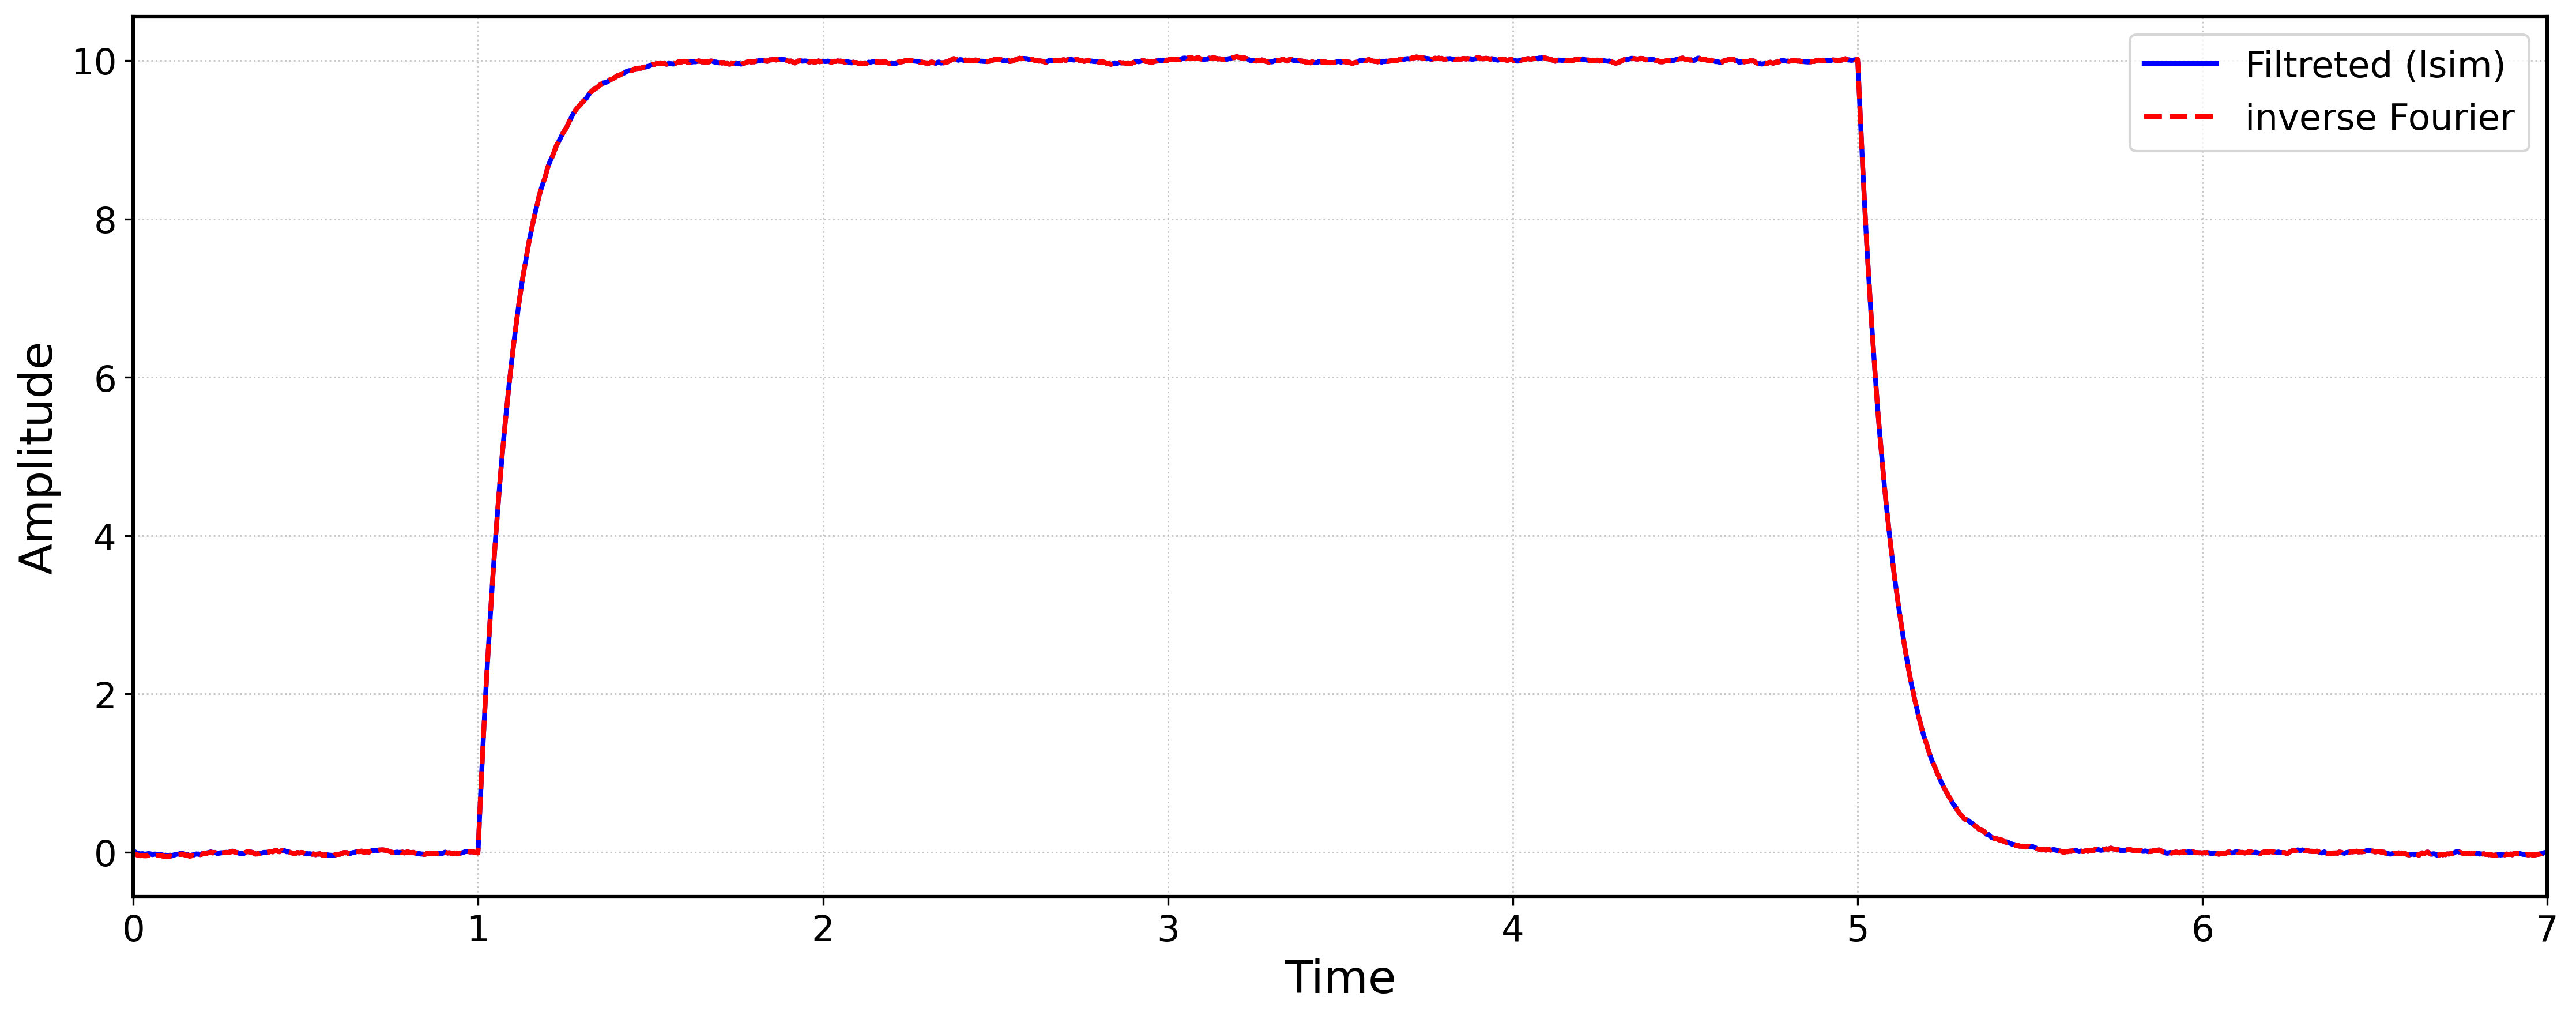
\includegraphics[width=1\textwidth]{../images/linearFilter/3.10.0.1.png}
		\caption{Сравнение методов фильтрации. \(a = 10, T = 0.1\)}  
		\label{fig:my_image}  
	\end{figure}
	
	\subsubsection{Сравнение модулей Фурье-образов сигналов}

Я построю сравнительные графики модулей Фурье-образов: $\lvert \hat{g}(\omega) \rvert$, $\lvert \hat{u}(\omega) \rvert$, $\lvert \hat{u}_{\text{фильтр}}(\omega) \rvert$.\\
	
	Зафиксирую параметр \(a = 4\) и буду менять параметр \(T\)
	\begin{figure}[H]  
		\centering
		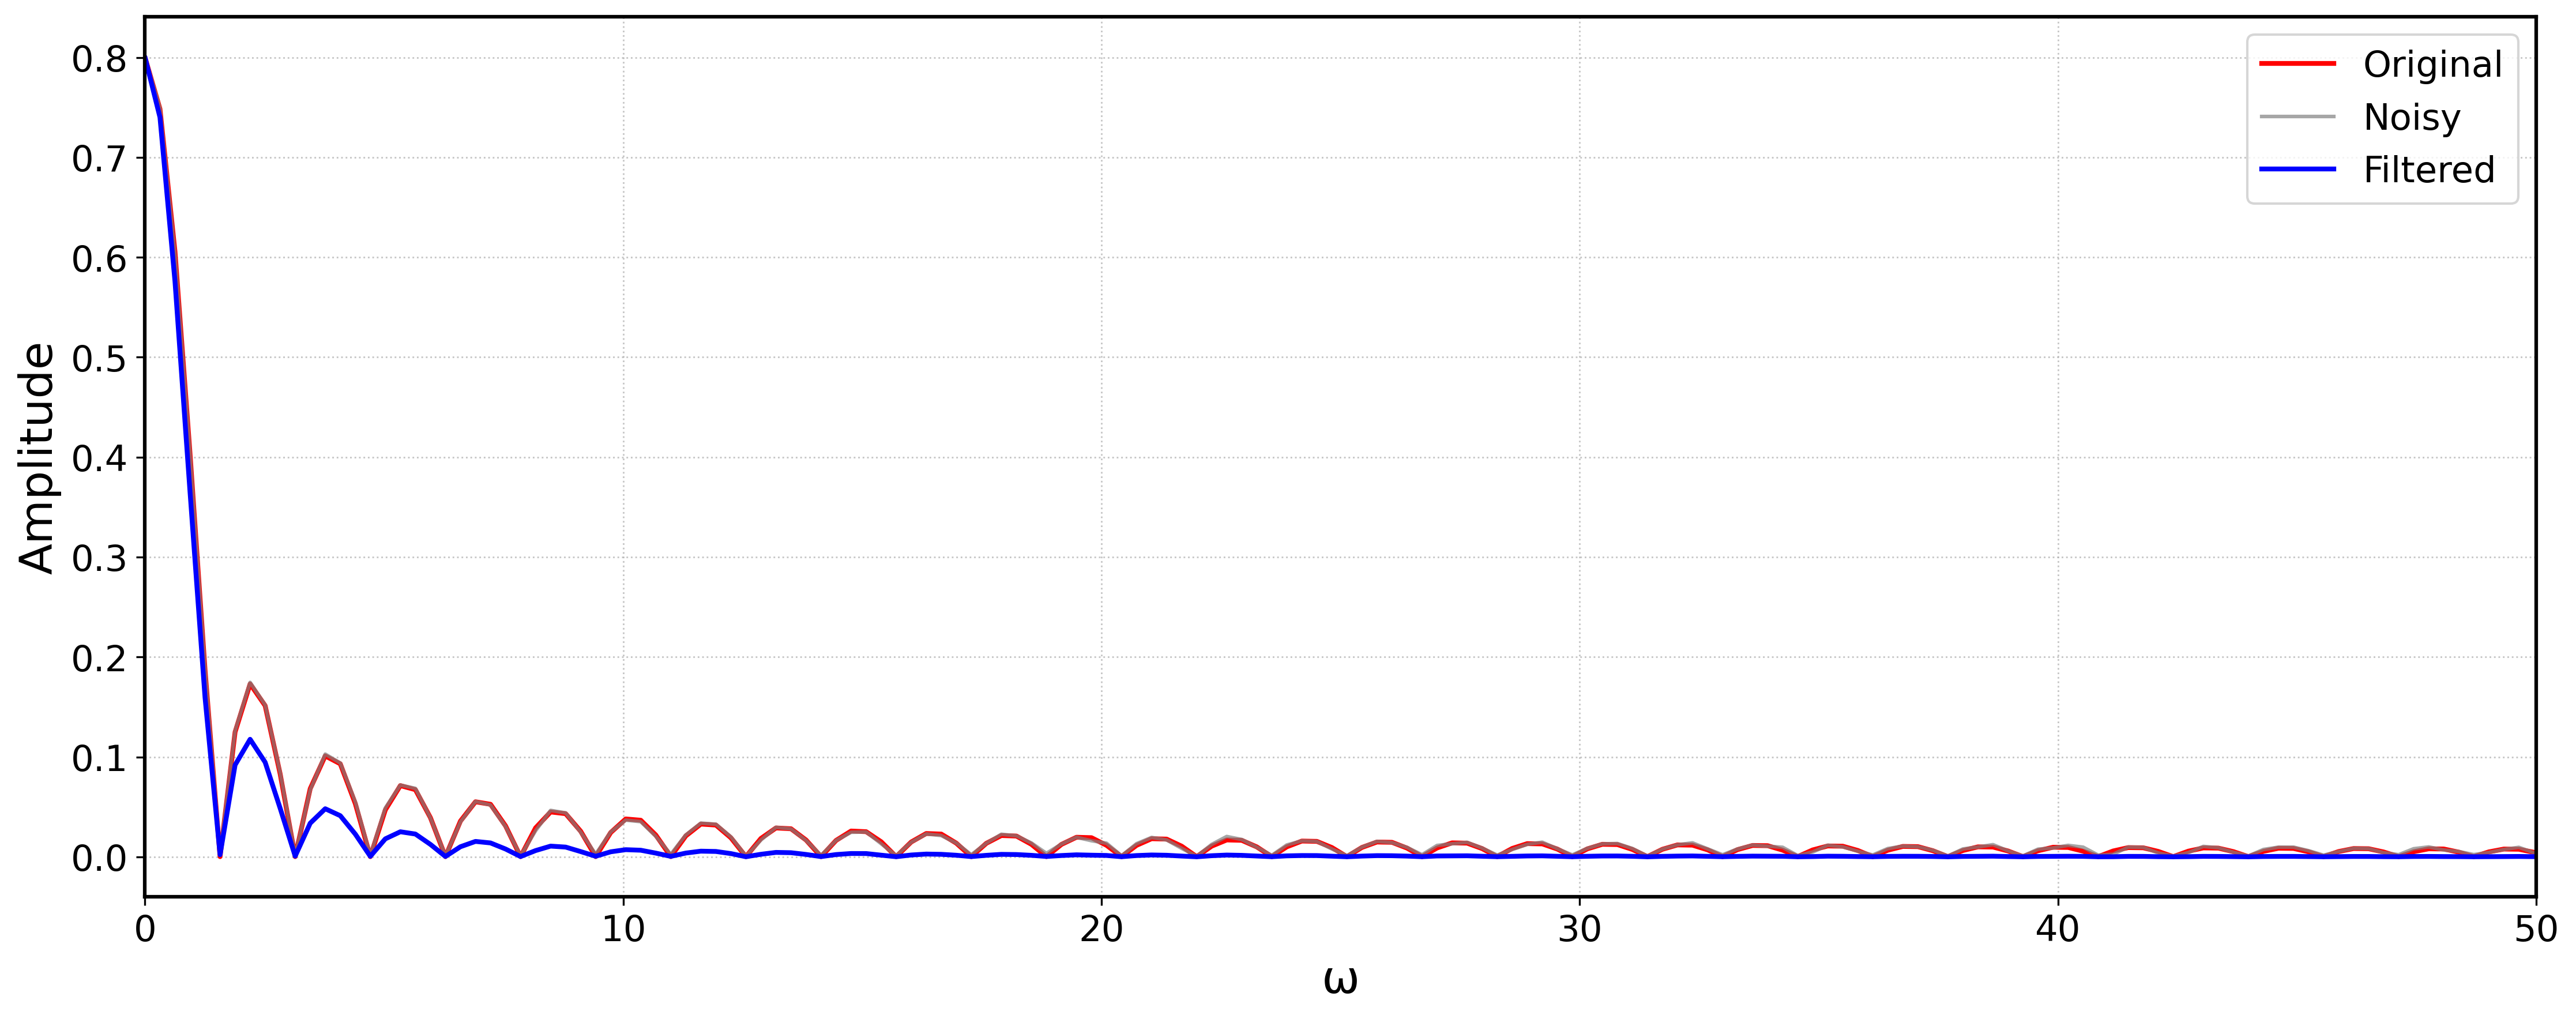
\includegraphics[width=1\textwidth]{../images/linearFilter/spectrum.4.05.png}
		\caption{Модули Фурье-образов. \(a = 4, T = 0.5\)}  
		\label{fig:my_image}  
	\end{figure}
	
	\begin{figure}[H]  
		\centering
		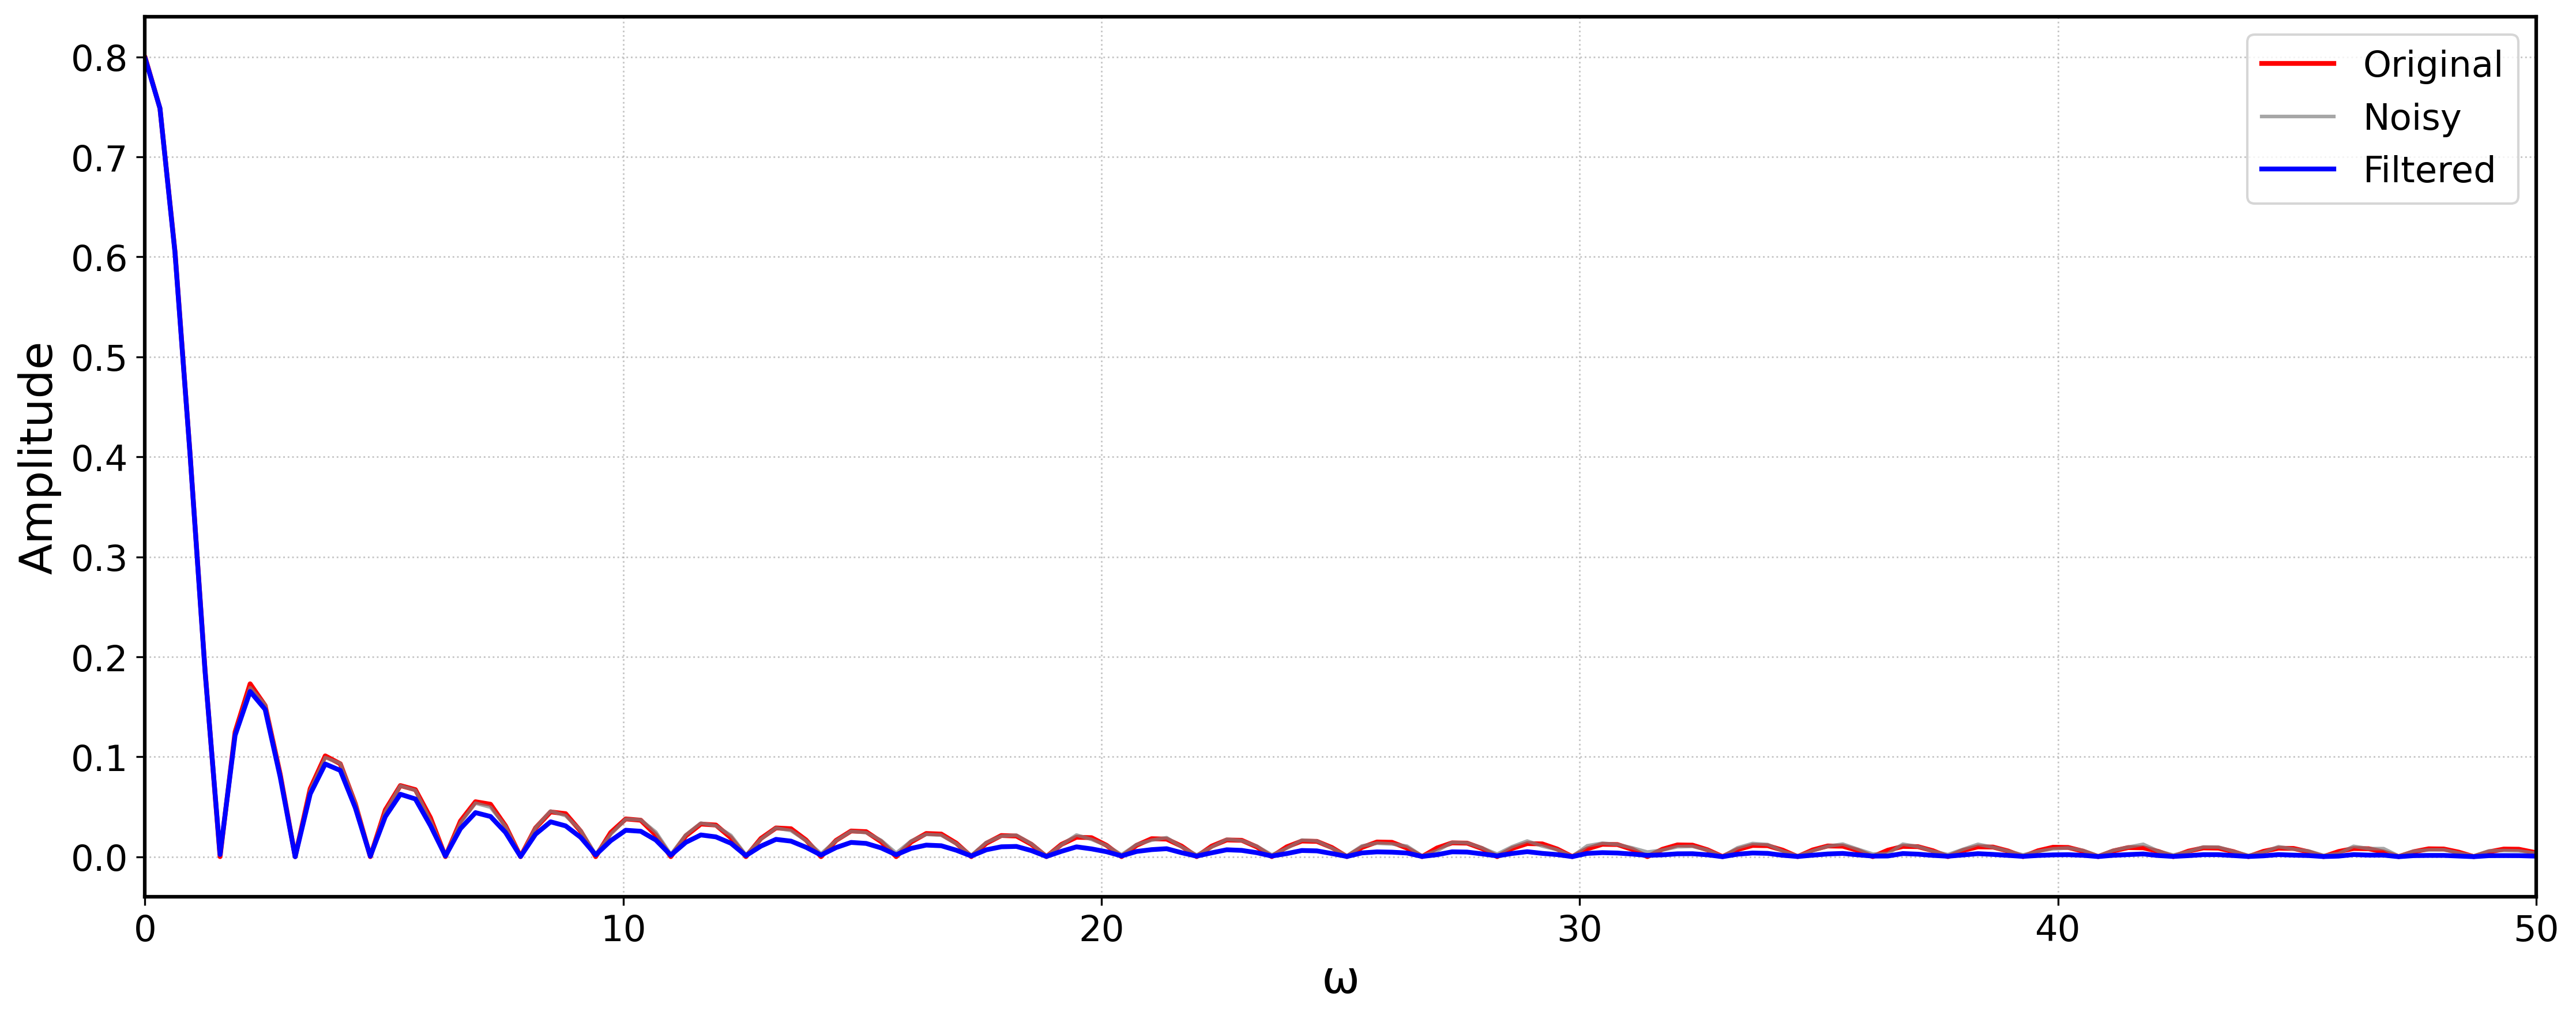
\includegraphics[width=1\textwidth]{../images/linearFilter/spectrum.4.0.1.png}
		\caption{Модули Фурье-образов. \(a = 4, T = 0.1\)}  
		\label{fig:my_image}  
	\end{figure}
	
	\begin{figure}[H]  
		\centering
		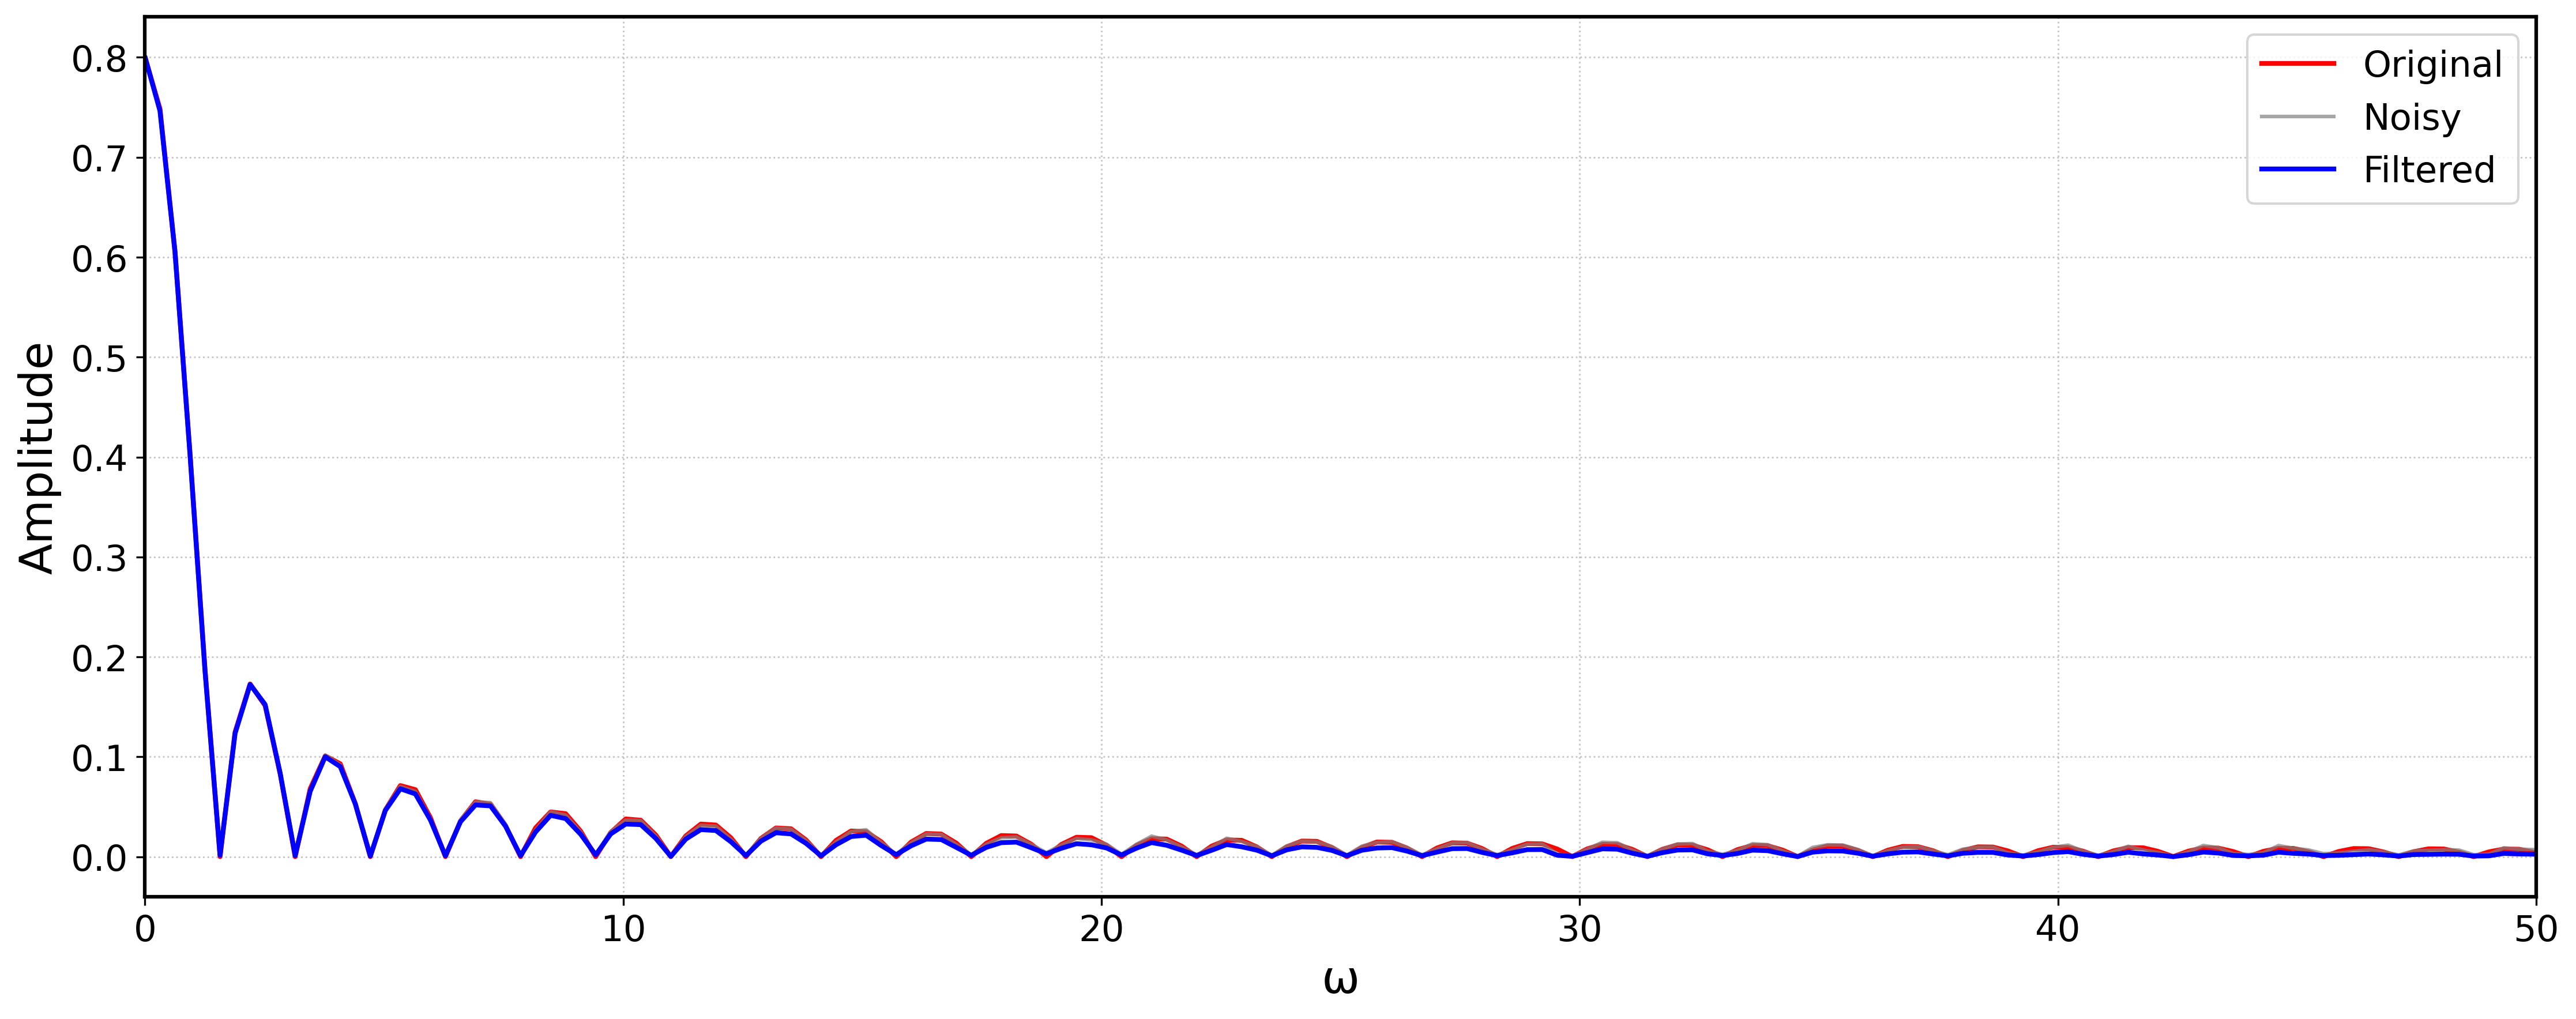
\includegraphics[width=1\textwidth]{../images/linearFilter/spectrum.4.0.05.png}
		\caption{Модули Фурье-образов. \(a = 4, T = 0.05\)}  
		\label{fig:my_image}  
	\end{figure}
	
	Зафиксирую параметр \(T = 0.1\) и буду менять параметр \(a\)
	
	\begin{figure}[H]  
		\centering
		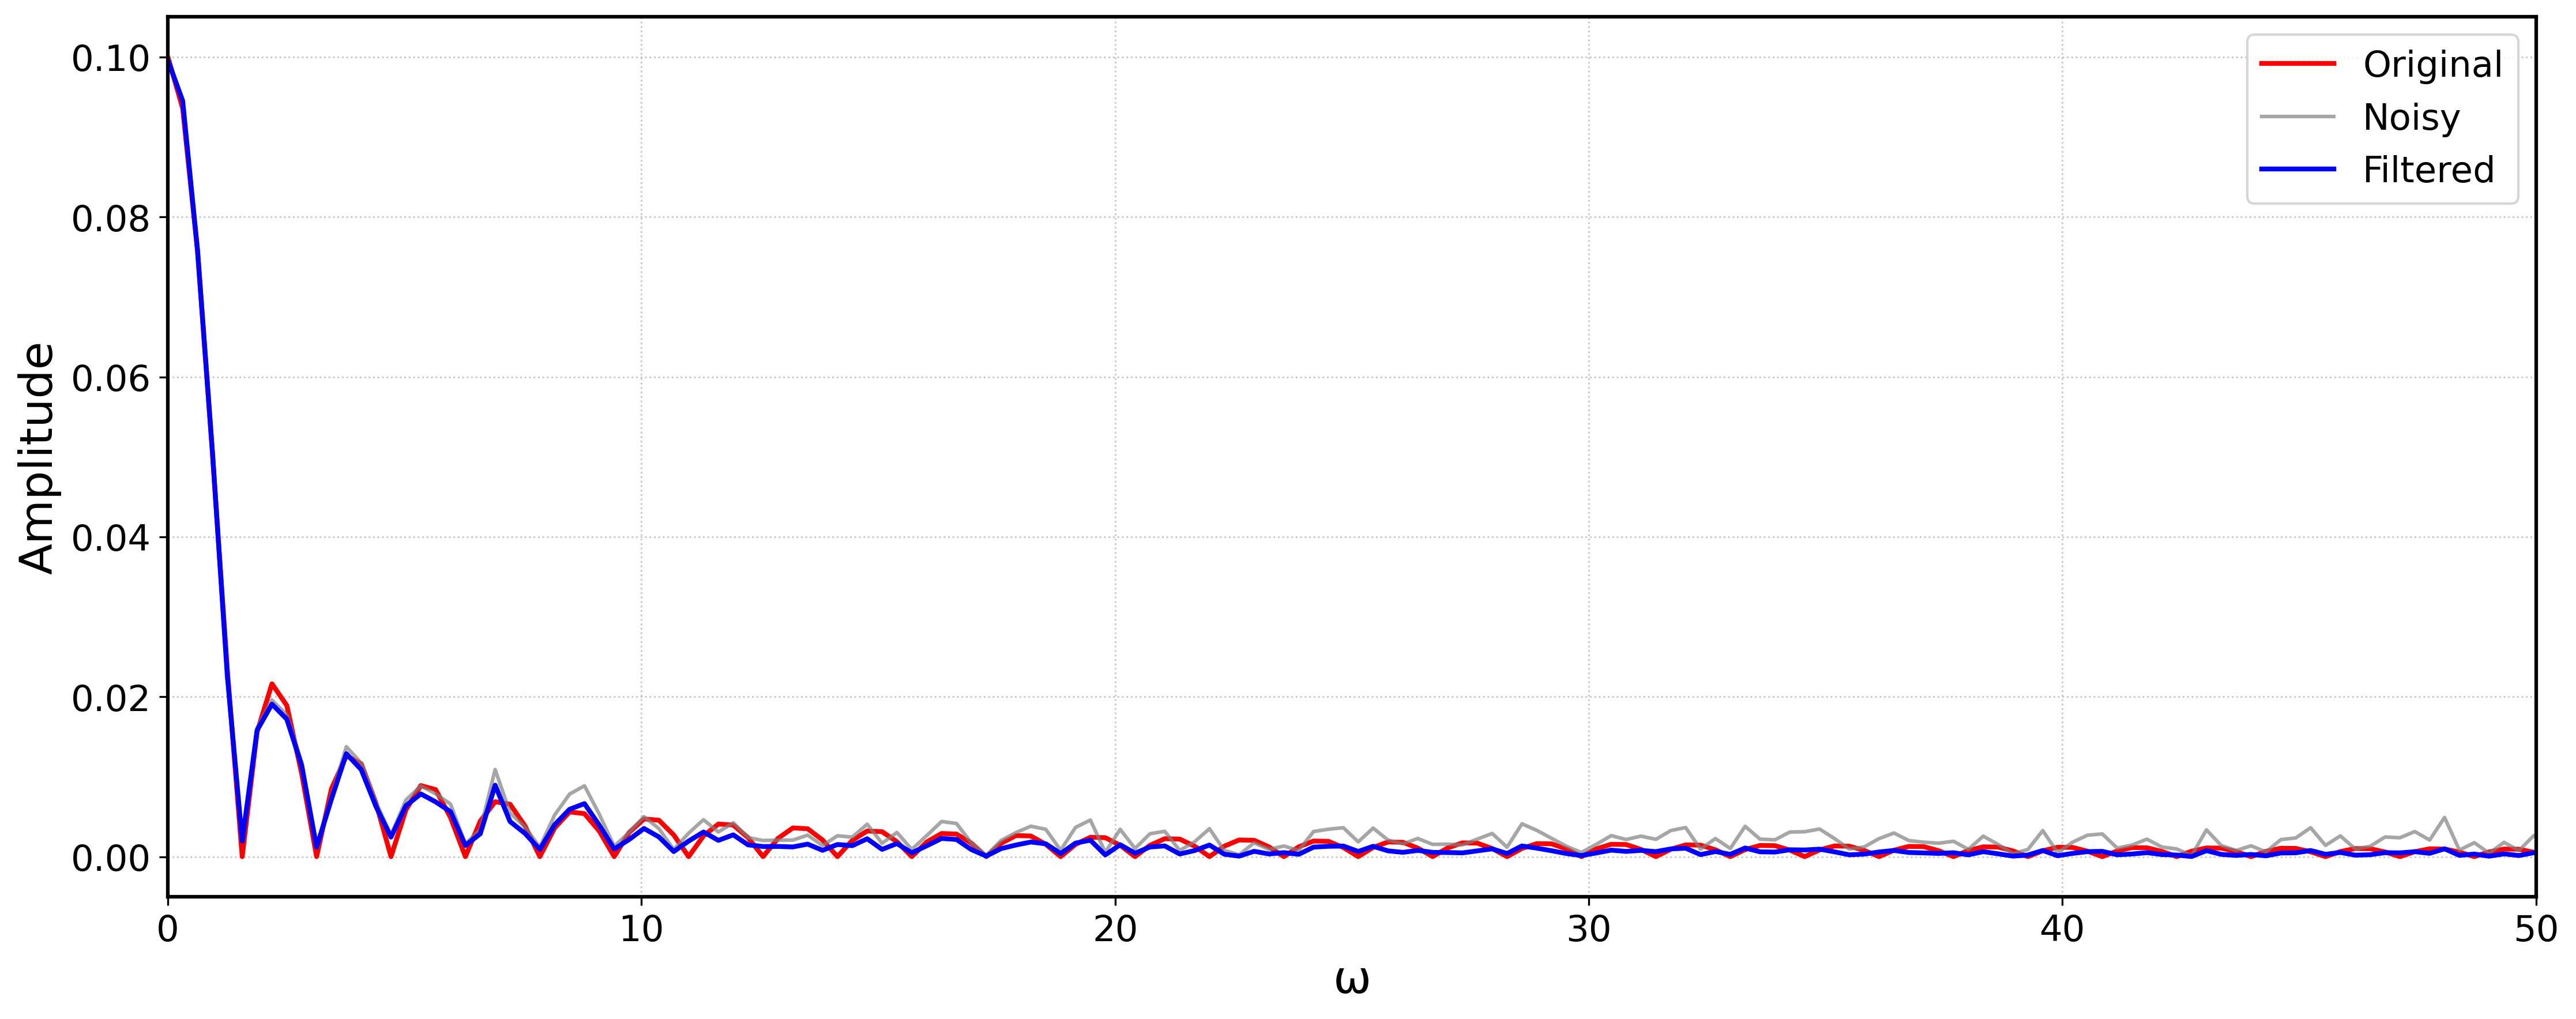
\includegraphics[width=1\textwidth]{../images/linearFilter/spectrum.0.5.0.1.png}
		\caption{Модули Фурье-образов. \(a = 0.5, T = 0.1\)}  
		\label{fig:my_image}  
	\end{figure}
	
	\begin{figure}[H]  
		\centering
		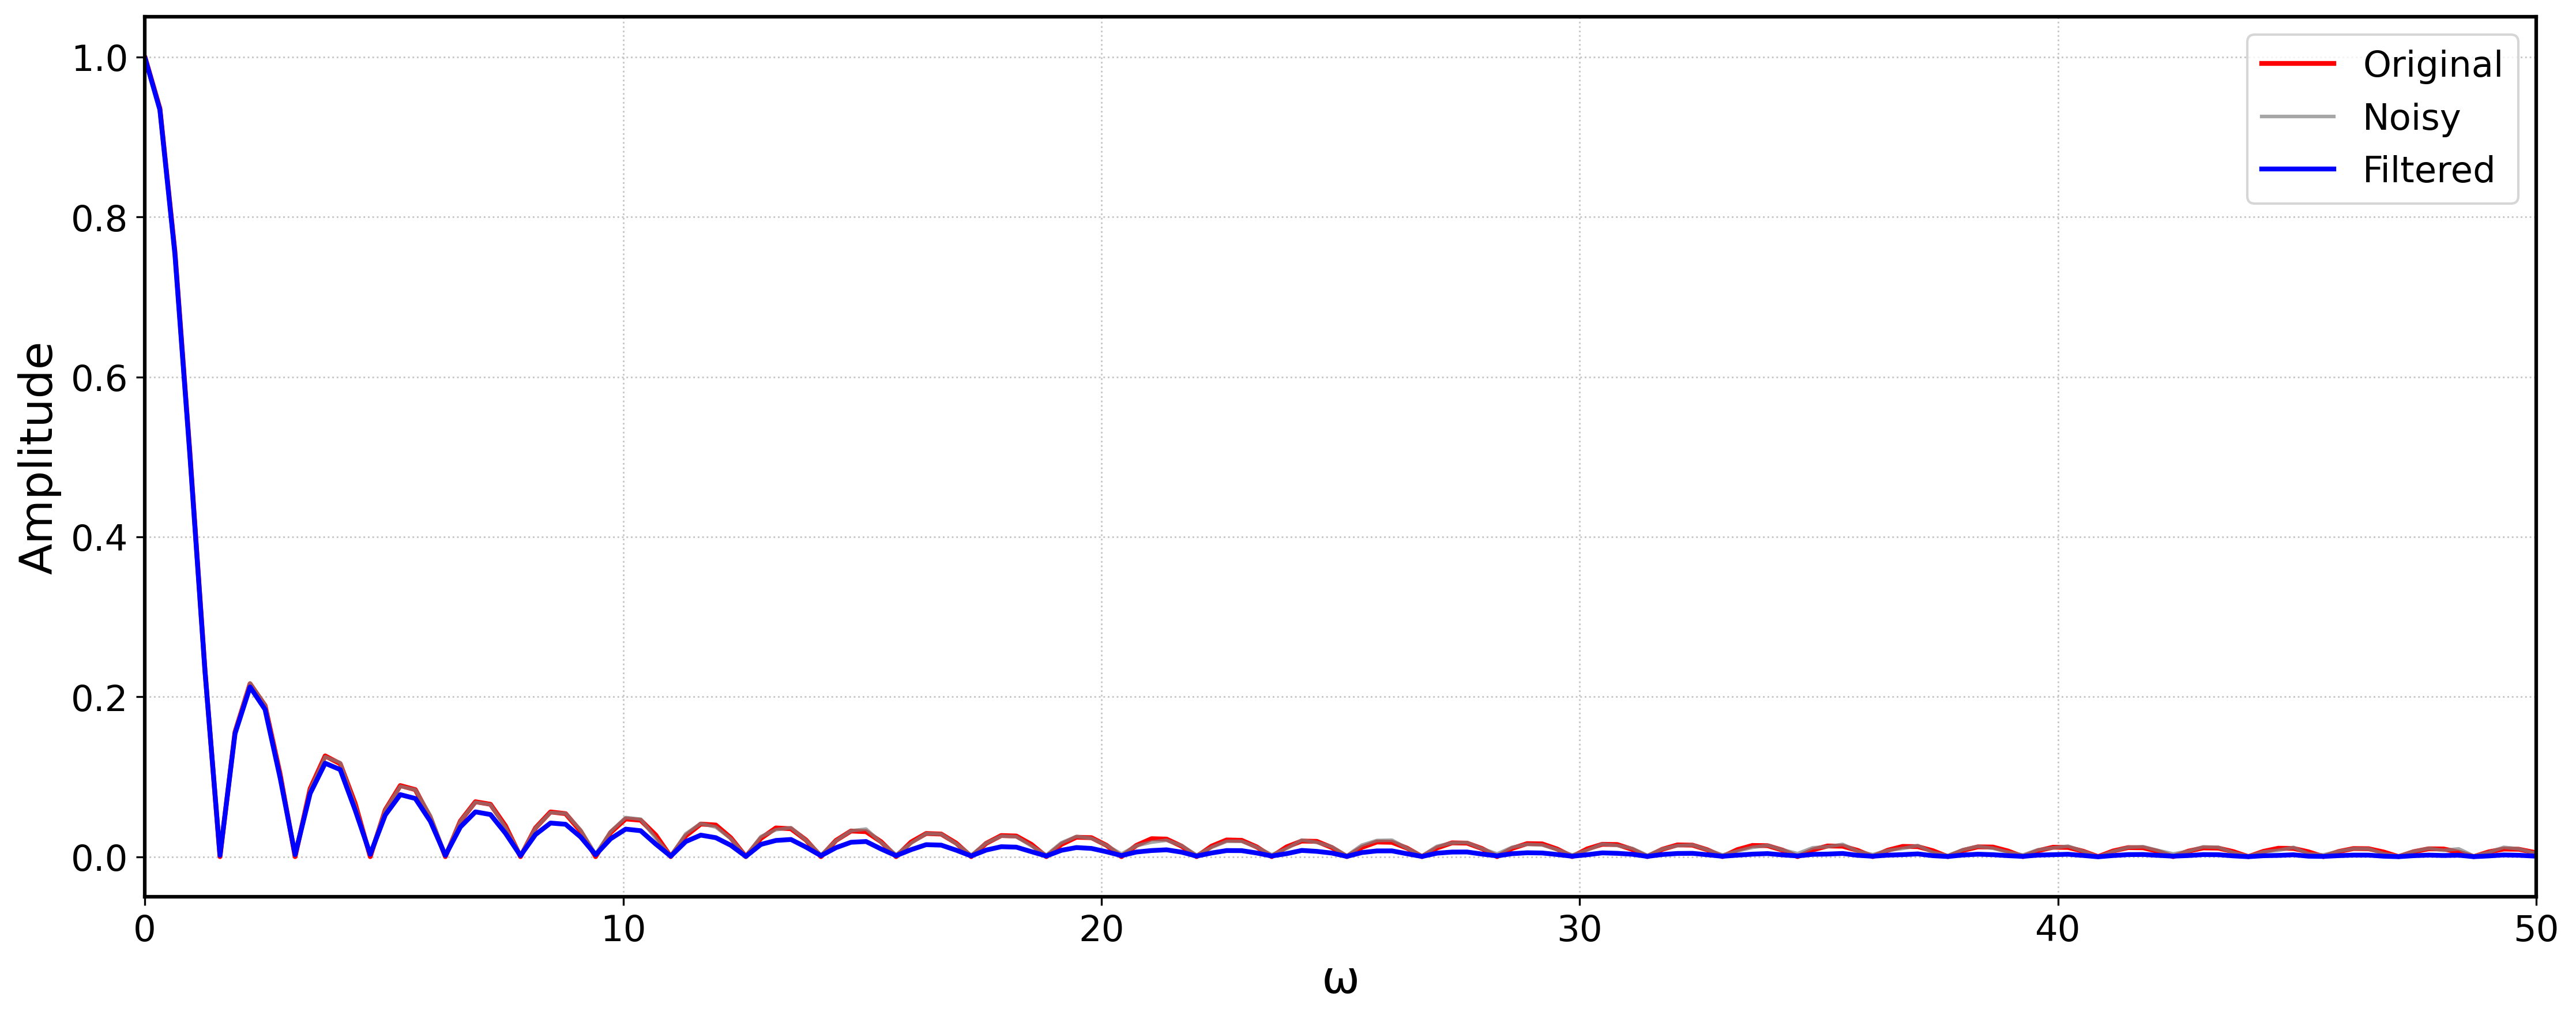
\includegraphics[width=1\textwidth]{../images/linearFilter/spectrum.5.0.1.png}
		\caption{Модули Фурье-образов. \(a = 5, T = 0.1\)}  
		\label{fig:my_image}  
	\end{figure}
	
	\begin{figure}[H]  
		\centering
		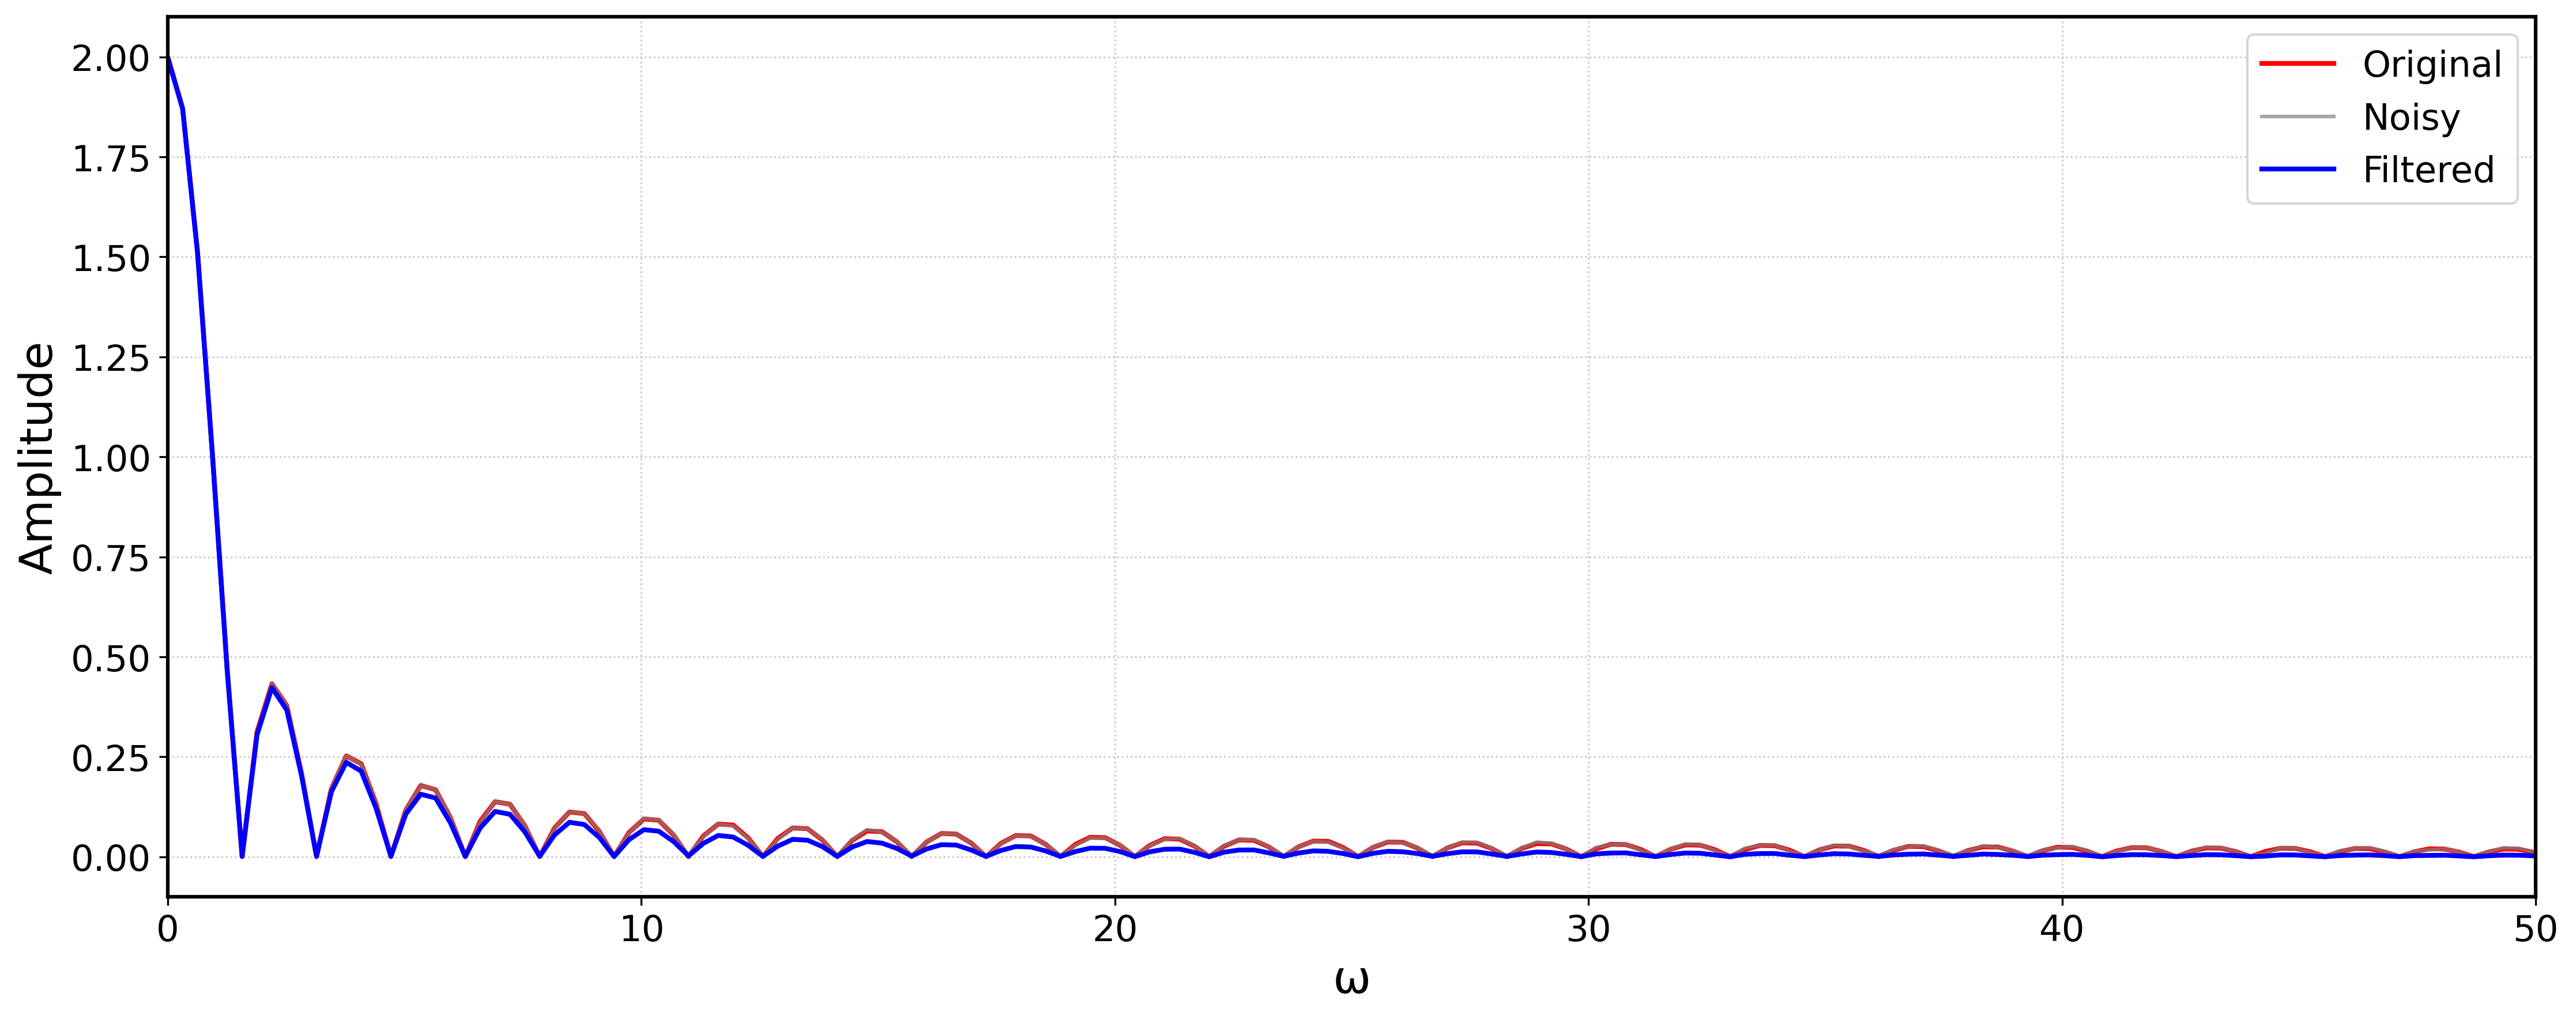
\includegraphics[width=1\textwidth]{../images/linearFilter/spectrum.10.0.1.png}
		\caption{Модули Фурье-образов. \(a = 10, T = 0.1\)}  
		\label{fig:my_image}  
	\end{figure}
	
	\subsubsection{Графики модулей Фурье-образа фильтрованного сигнала и \(W_1(i\omega)\cdot \hat{u}(\omega)\)}
	
	Построю графики  
	\[
	\begin{cases}
		|\hat{u}_{\text{фильтр}}(\omega)| & \text{--- спектр фильтрованного сигнала} \\
		|W_1(i\omega)\hat{u}(\omega)| & \text{--- произведение АЧХ и спектра зашумленного сигнала}
	\end{cases}
	\]\\
	
	Зафиксирую параметр \(a = 4\) и буду менять параметр \(T\)
	\begin{figure}[H]  
		\centering
		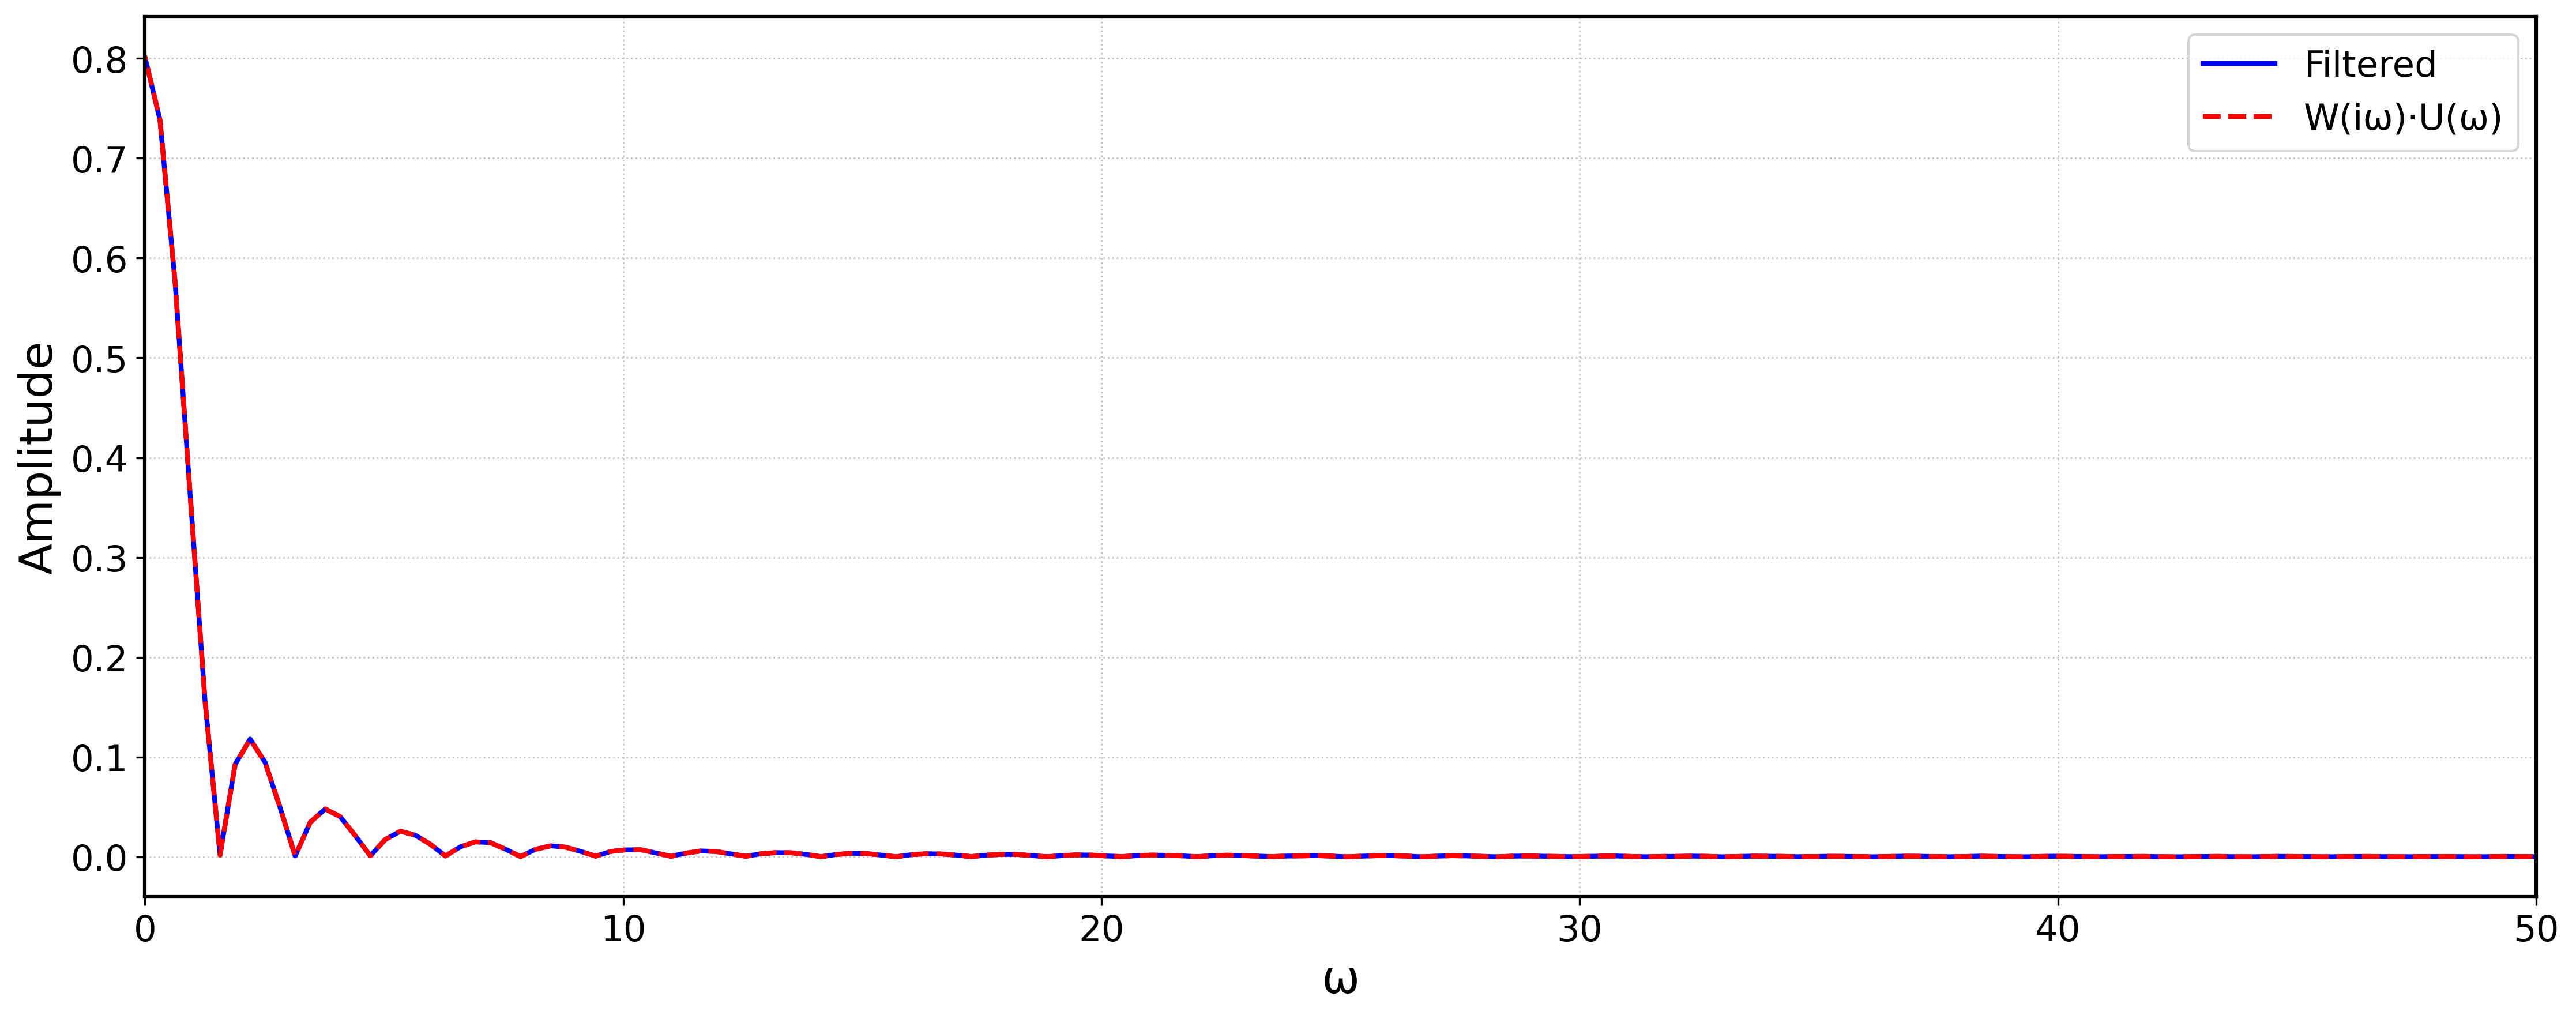
\includegraphics[width=1\textwidth]{../images/linearFilter/methods.4.05.png}
		\caption{Сравнение методов. \(a = 4, T = 0.5\)}  
		\label{fig:my_image}  
	\end{figure}
	
	\begin{figure}[H]  
		\centering
		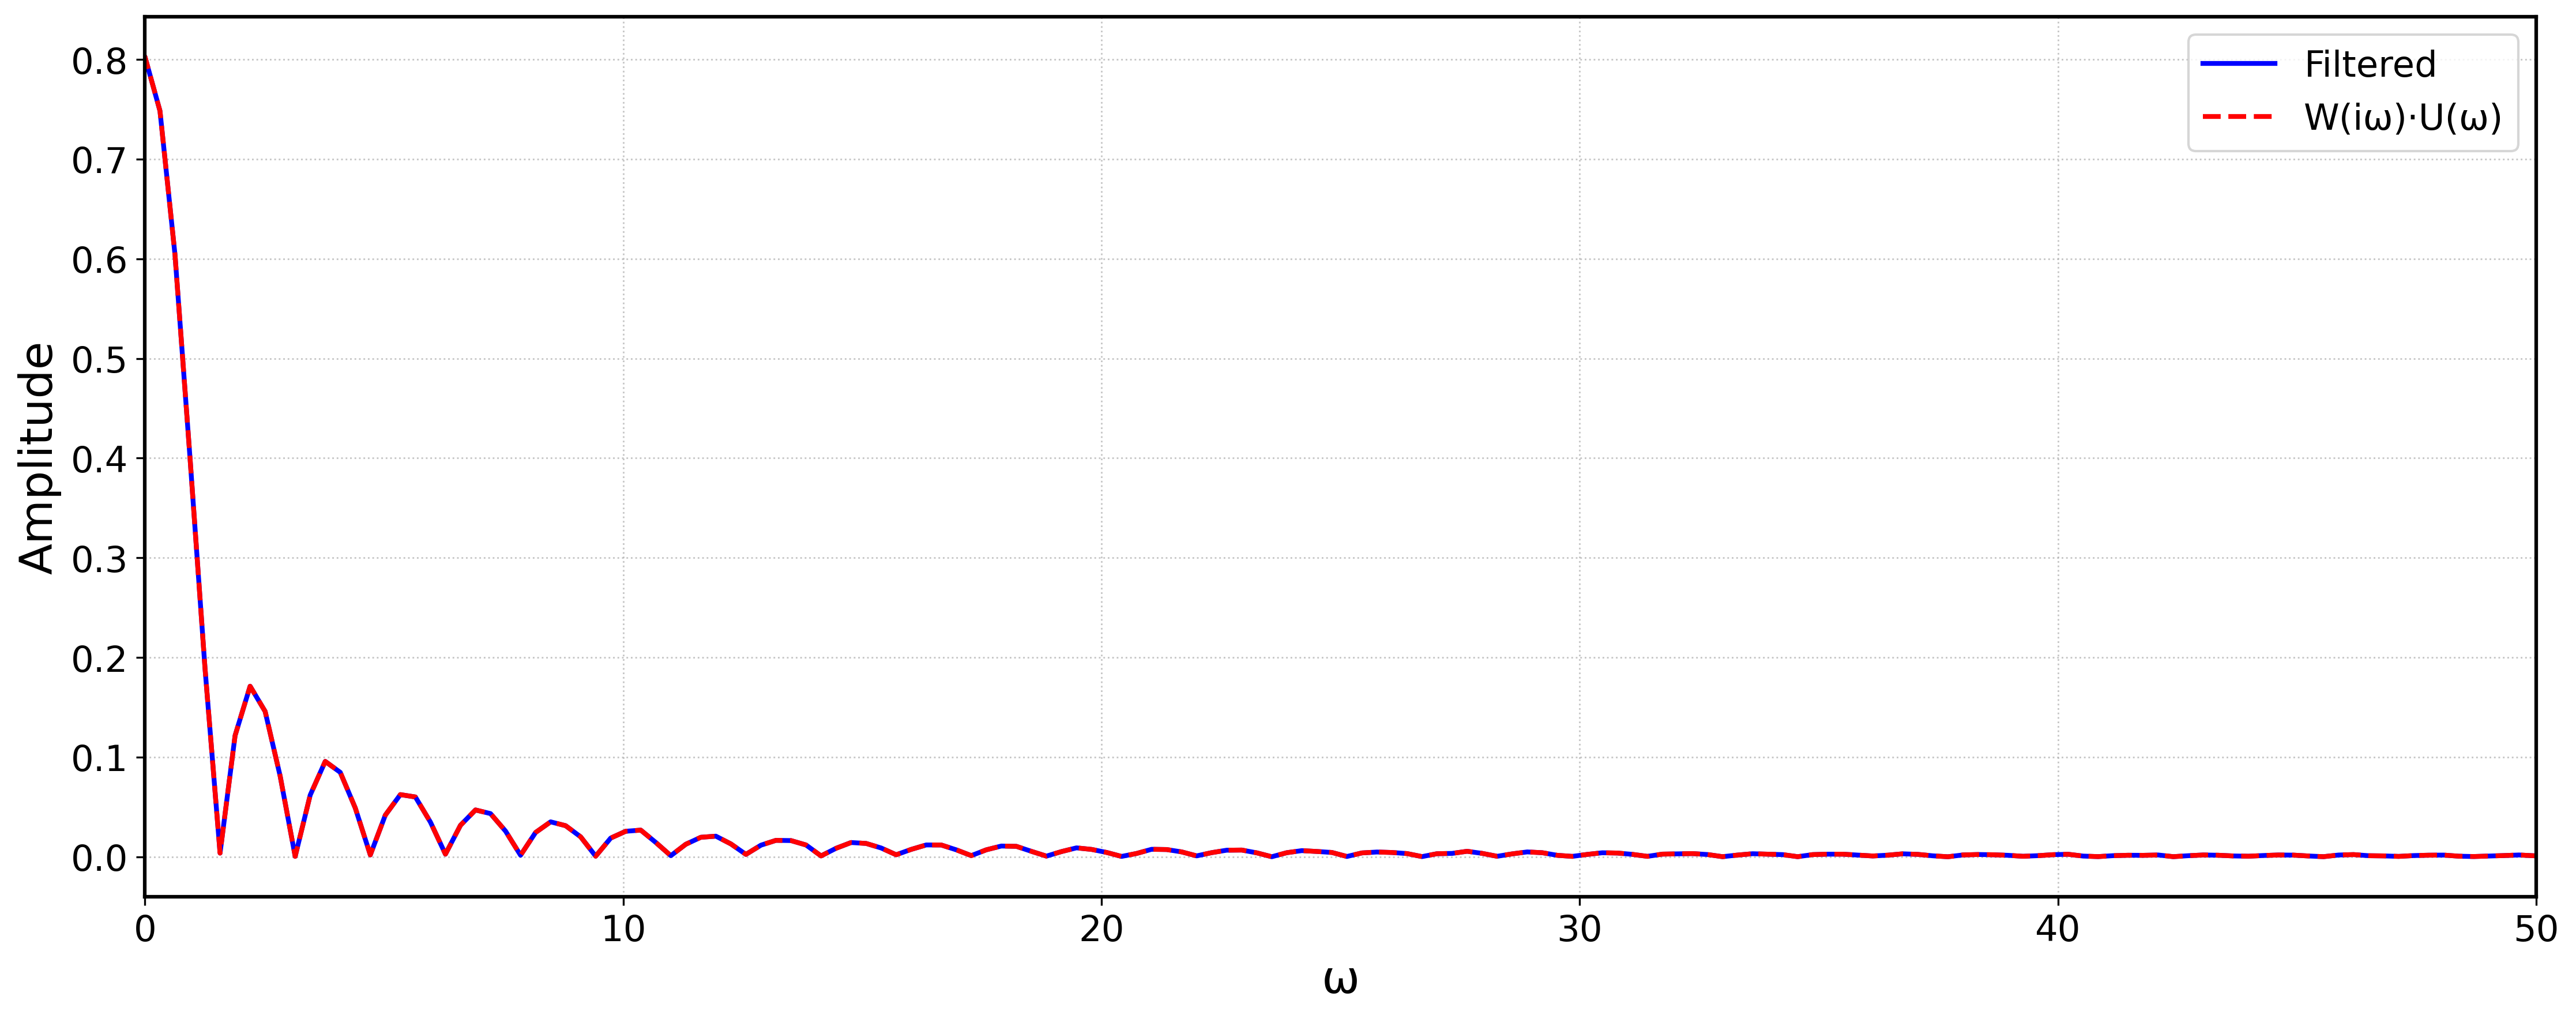
\includegraphics[width=1\textwidth]{../images/linearFilter/methods.4.0.1.png}
		\caption{Сравнение методов. \(a = 4, T = 0.1\)}  
		\label{fig:my_image}  
	\end{figure}
	
	\begin{figure}[H]  
		\centering
		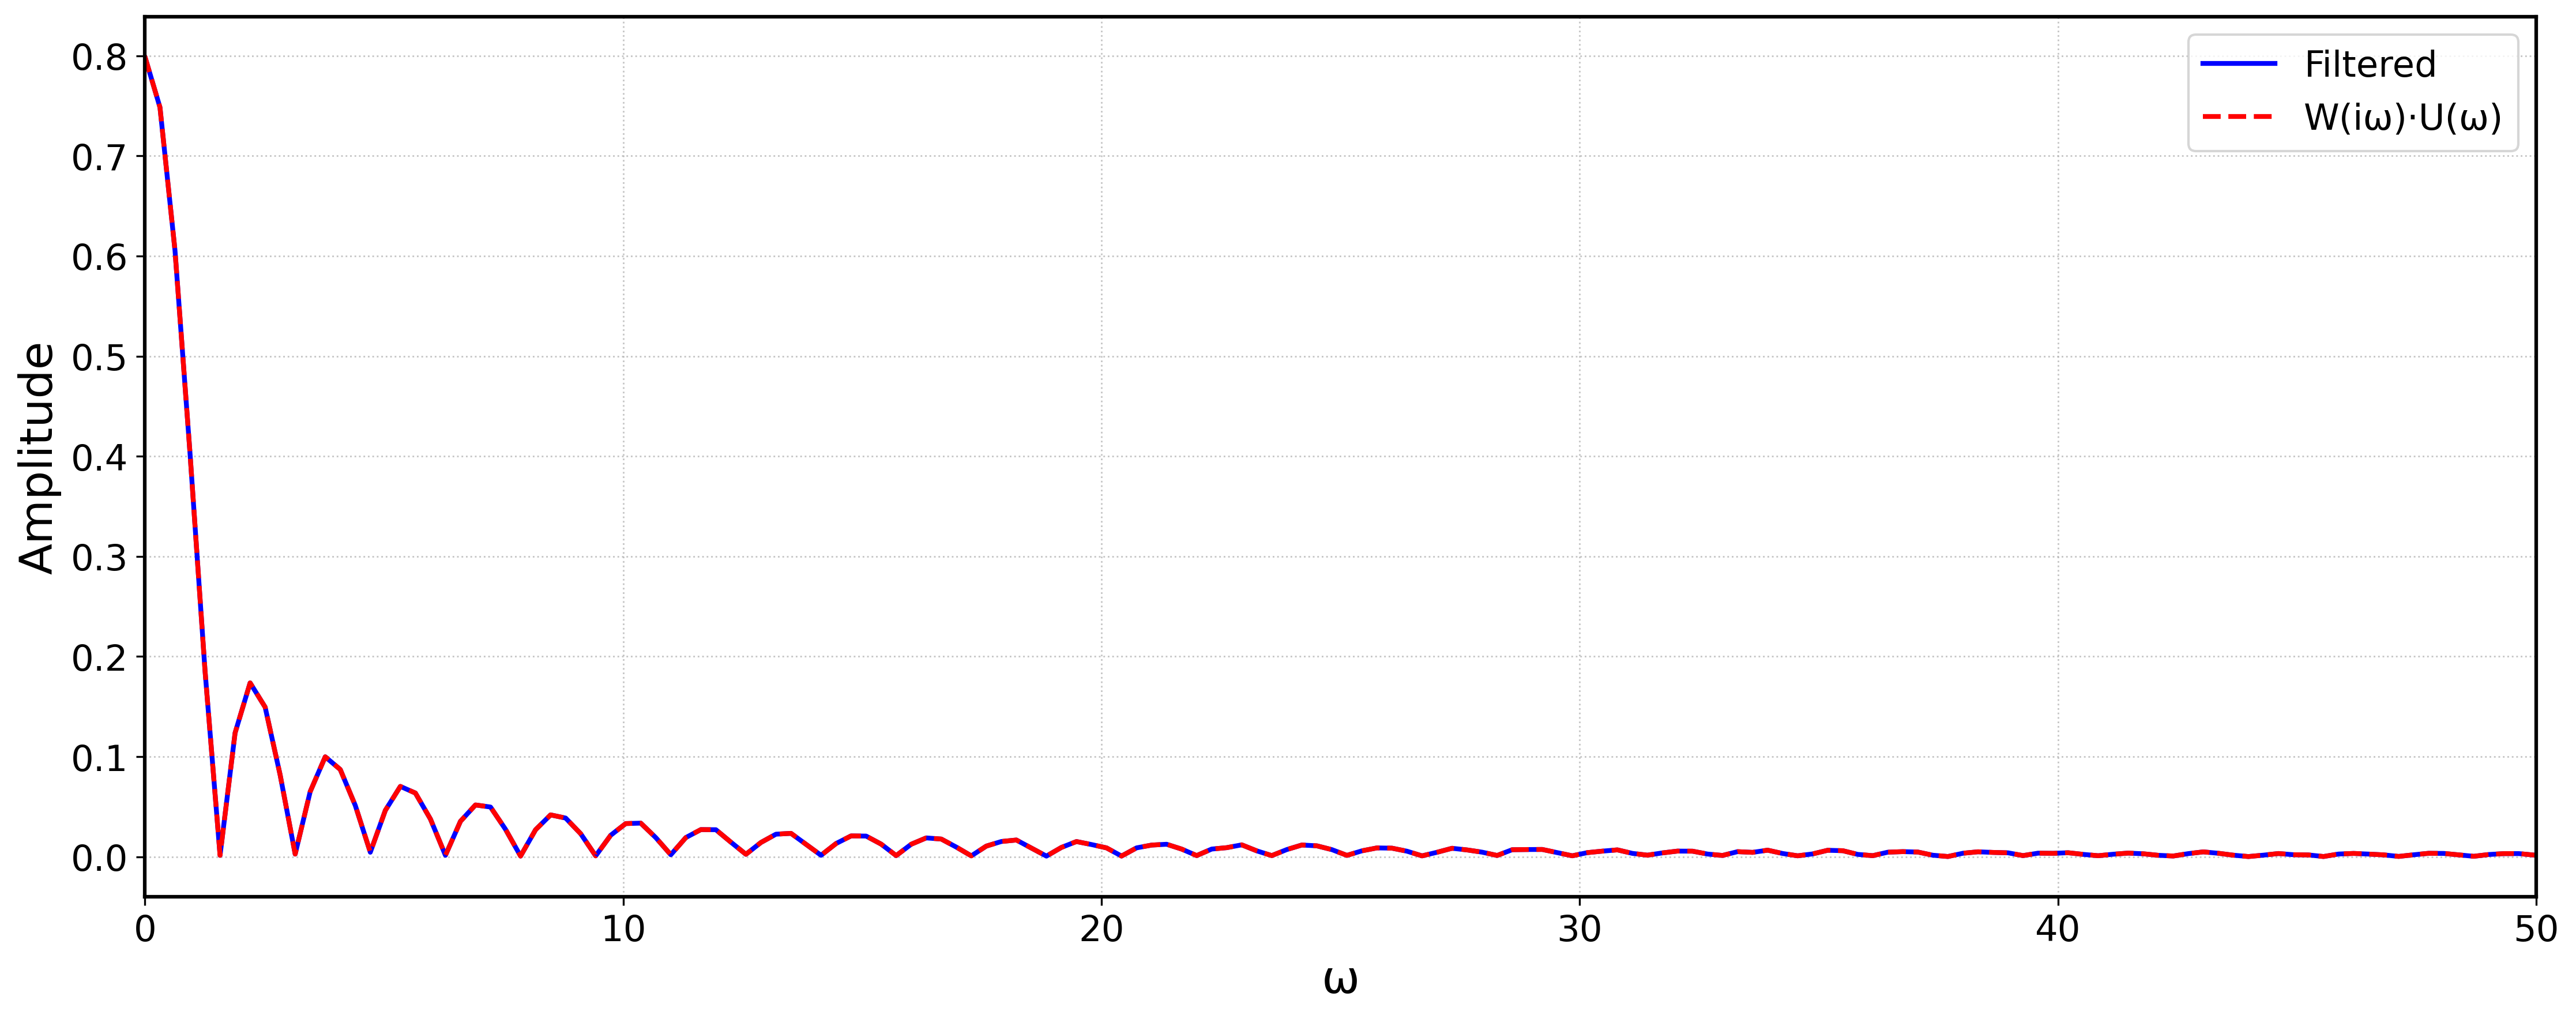
\includegraphics[width=1\textwidth]{../images/linearFilter/methods.4.0.05.png}
		\caption{Сравнение методов. \(a = 4, T = 0.05\)}  
		\label{fig:my_image}  
	\end{figure}
	
	Зафиксирую параметр \(T = 0.1\) и буду менять параметр \(a\)
	
	\begin{figure}[H]  
		\centering
		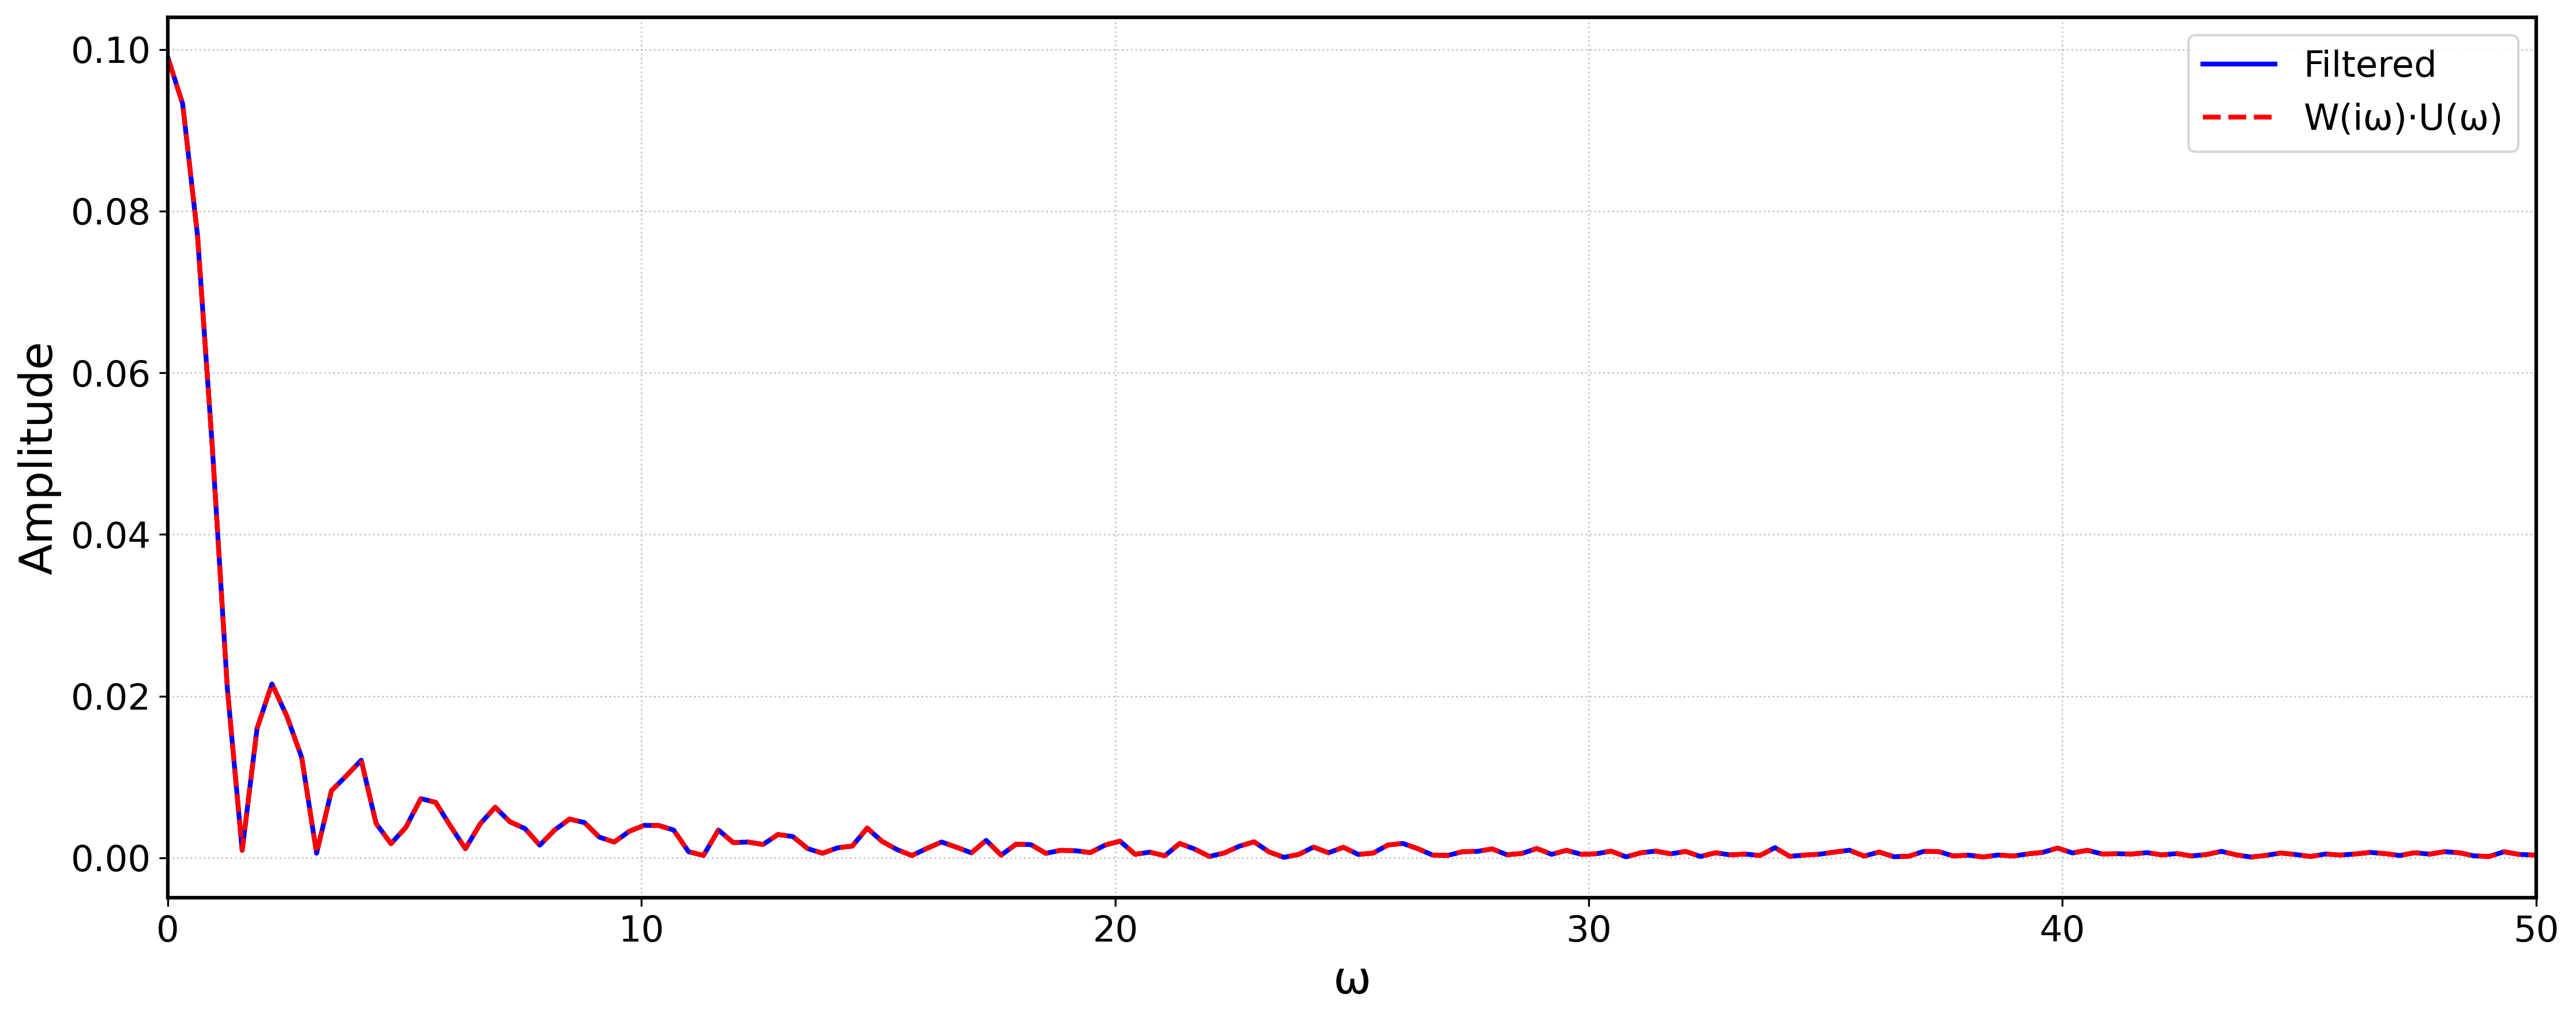
\includegraphics[width=1\textwidth]{../images/linearFilter/methods.0.5.0.1.png}
		\caption{Сравнение методов. \(a = 0.5, T = 0.1\)}  
		\label{fig:my_image}  
	\end{figure}
	
	\begin{figure}[H]  
		\centering
		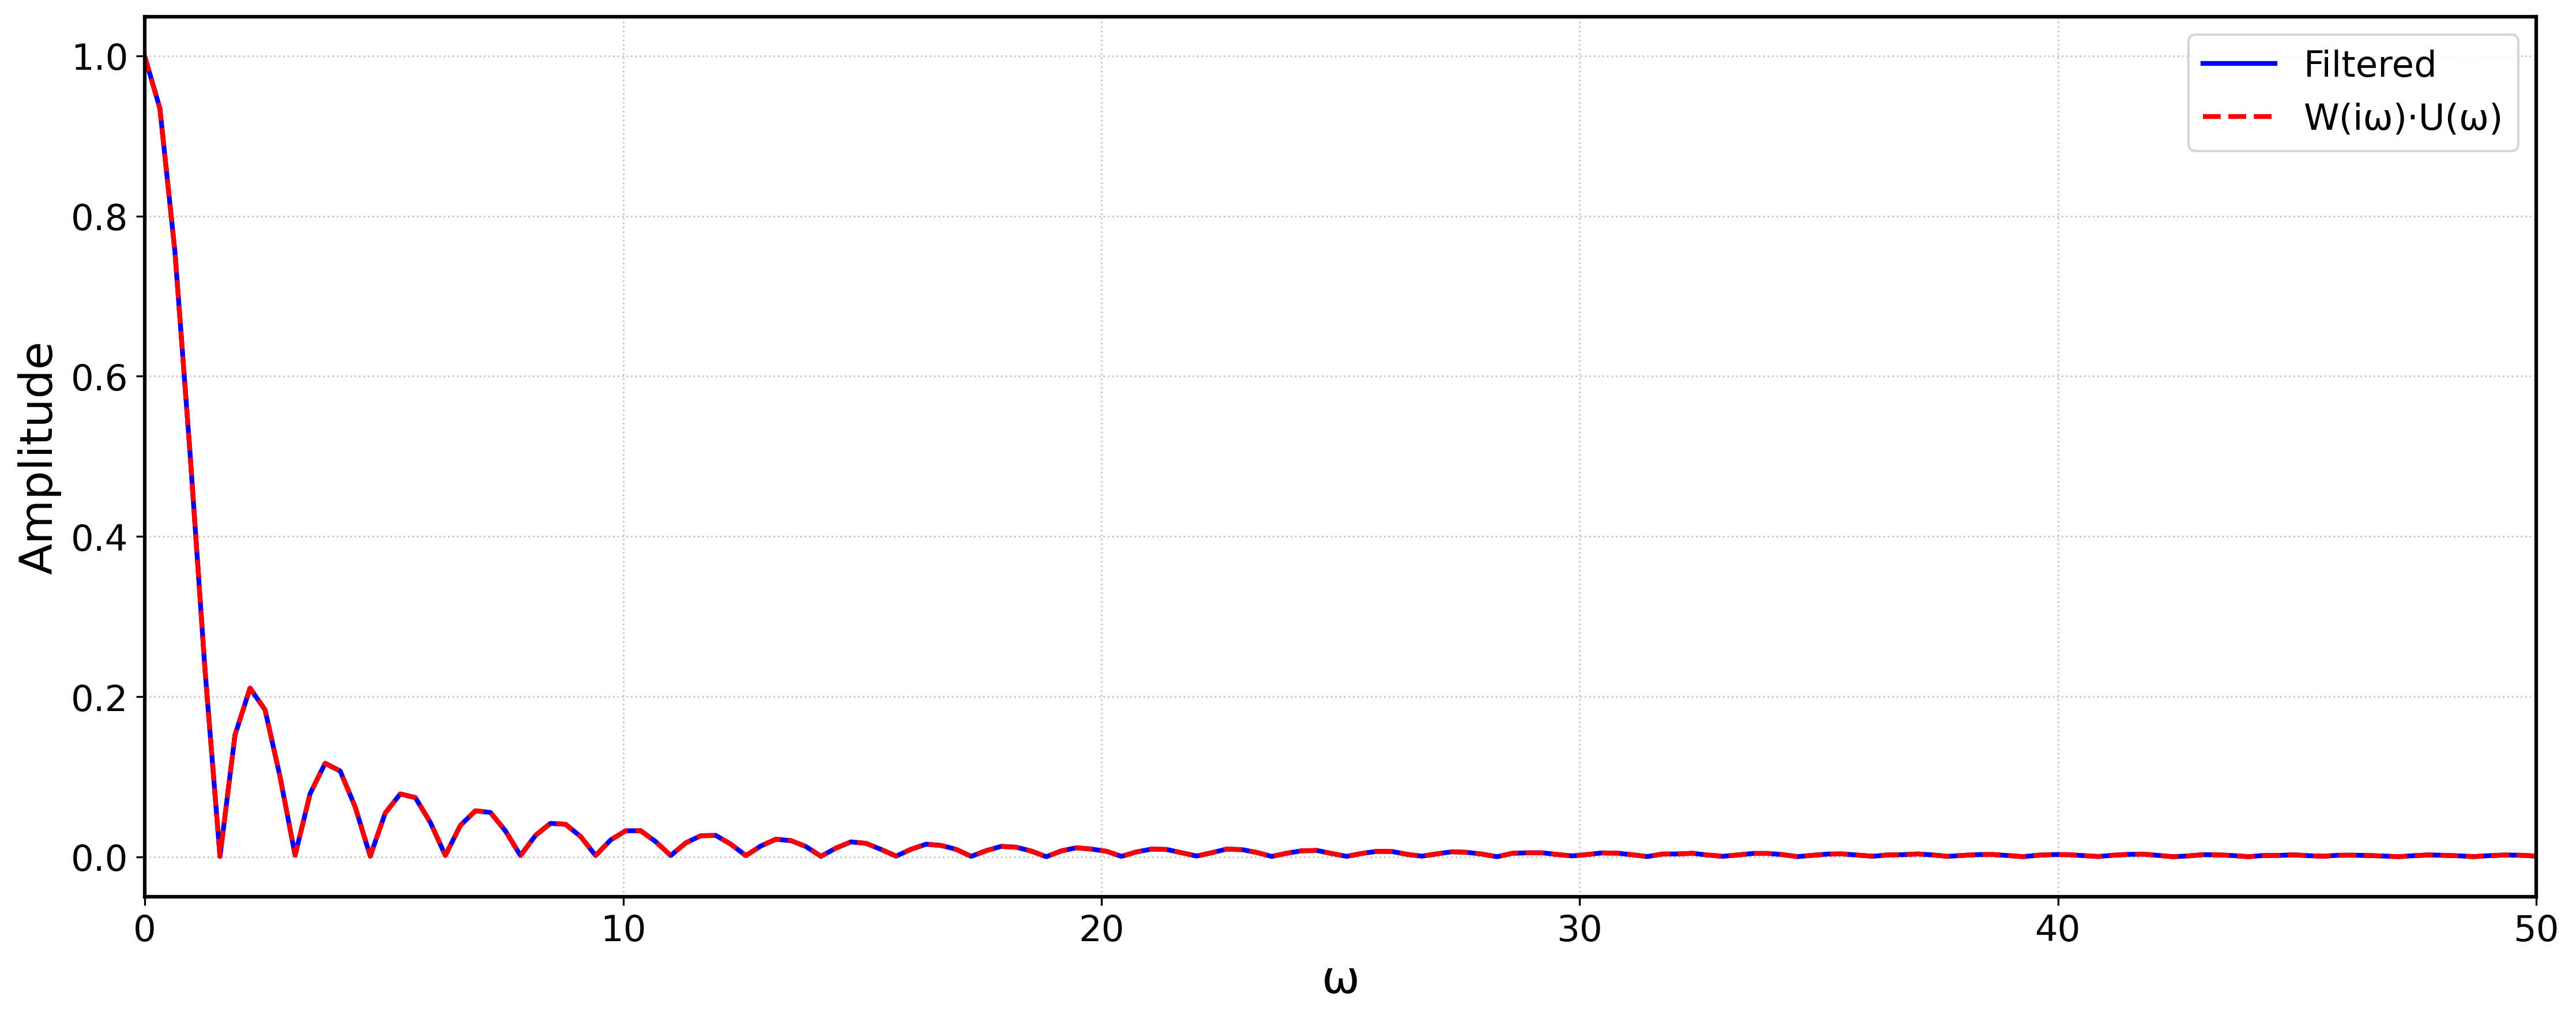
\includegraphics[width=1\textwidth]{../images/linearFilter/methods.5.0.1.png}
		\caption{Сравнение методов. \(a = 5, T = 0.1\)}  
		\label{fig:my_image}  
	\end{figure}
	
	\begin{figure}[H]  
		\centering
		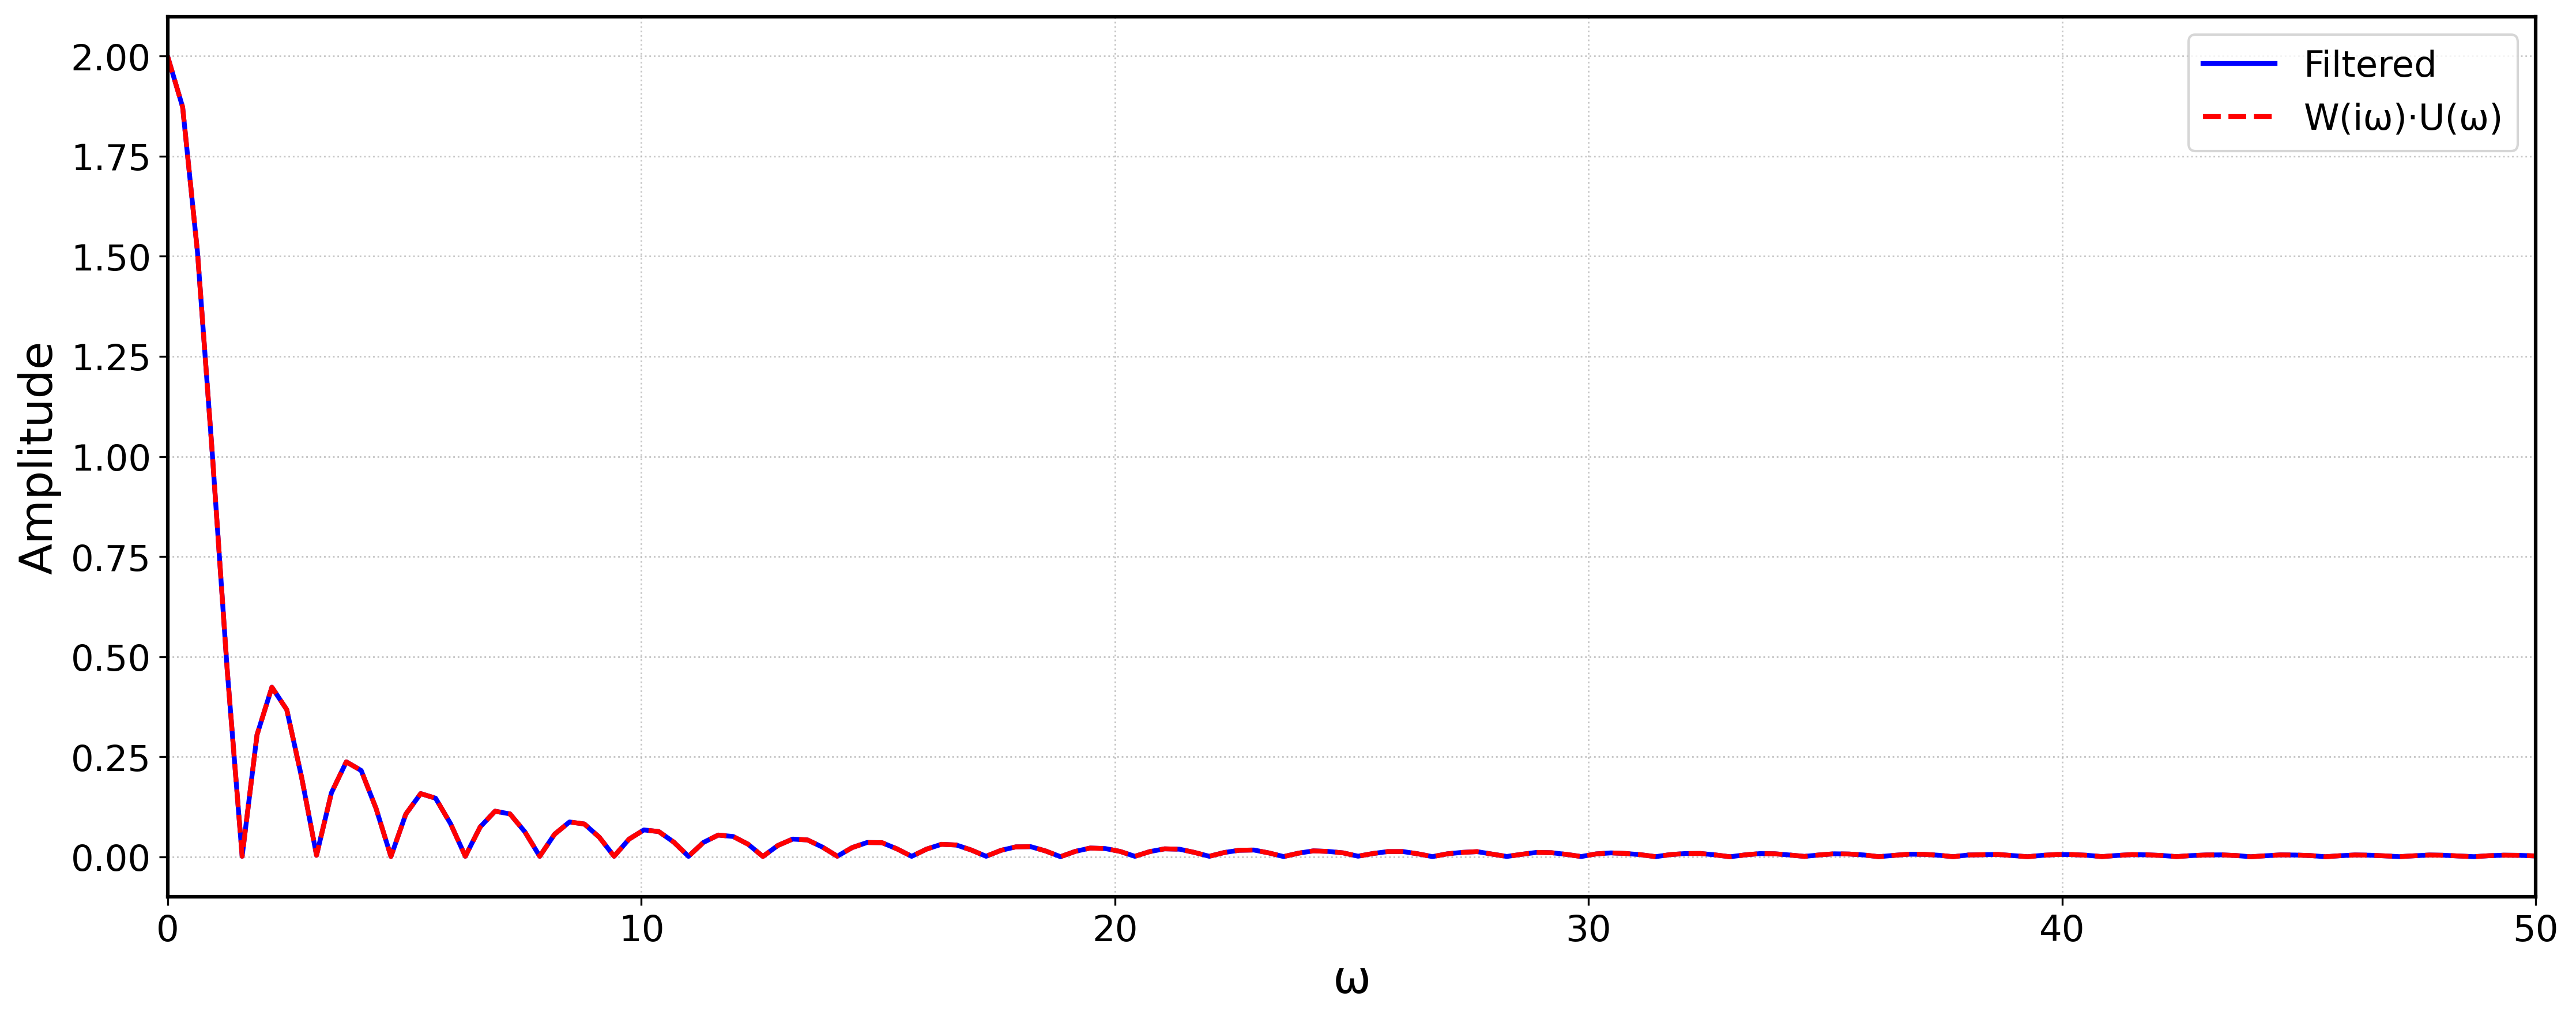
\includegraphics[width=1\textwidth]{../images/linearFilter/methods.10.0.1.png}
		\caption{Сравнение методов. \(a = 10, T = 0.1\)}  
		\label{fig:my_image}  
	\end{figure}
	
	\subsubsection{Выводы}
	
	
	
	
	
	
	
	
	
	
	
	
	
\end{document}
